\chapter{Background and Related Work}

%\section{Terminology \ar Glossary?}
%
%\paragraph{Planar image}
%\paragraph{360\degree image} vs panorama
%\paragraph{Interpolation vs Synthesis} In the context of this thesis, the two terms are very similar. Interpolation is used as a type of synthesis where two images are weighted by a certain amount and added together \ldots ?
%\paragraph{Viewpoint, capture, camera} input viewpoint, output viewpoint
%Capture/Viewpoint is the term used here to signify the location and image data of a 360\degree photograph taken at a certain position in the scene
%capture is more for when the images are actually recorded
%viewpoint is more for during processing
%\paragraph{UV coordinates}
%image-based rendering vs pixel-based rendering

%\section{Fundamentals of 360\degree Images}
\section{Fundamentals}
Before diving into image-based rendering techniques in general and the pixel-based synthesis presented in this thesis, it is important to understand some basic concepts and methods used. Since 360\degree images are used throughout, it is important to understand how such images are created and how the data can be visualized on a planar surface. Furthermore, the concept of optical flow is introduced, as it is utilized in the pixel-based synthesis.

\subsection{360\degree Images}\label{subsec:fundamentals_360}
Capturing an image with a 360\degree camera can be regarded mathematically as a series of projections. The sensors of a 360\degree camera can be simplified as a unit sphere covered in light receptors, where the number of light receptors corresponds to the resolution of the camera. This means that the complete surroundings are projected onto this sphere by way of incoming light rays. The limited number of sensors acts as a discretizer and captures a specific color value for each sampling point (pixel). At this point, the data is in \emph{world coordinates}, meaning that each pixel value corresponds to a point on the surface of the unit sphere. 
%\missingfigure{incoming light rays on unit sphere, maybe with uv indices \label{fig:lightrays}}

\subsubsection{UV Mapping for Spherical Geometry}
As the majority of viewing devices are planar (e.g. computer or smartphone screens), the image data needs to be projected to a flat surface in order to be viewed on a flat screen. This problem is known in computer graphics as \emph{uv mapping} or \emph{texture mapping}, and it describes the process that translates the data from world coordinates to \emph{image coordinates} and vice versa.

The pixel values in image coordinates (uv) are associated with the world coordinates (x,y,z) by a bijective mapping function. Figure~\ref{fig:uv_mapping} shows an example mapping between the unit sphere and an equirectangular image. In this example, the poles of the sphere are mapped to the entire top and bottom of the image, which means that the mapping function is not \emph{equal area} i.e. it does not conserve how much area a color value occupies. Often the image values are some type of color values, however, other kinds of information can be uv-mapped to a shape, for example illumination data, depth values (bump mapping), and more.

\begin{figure}
		\centering
		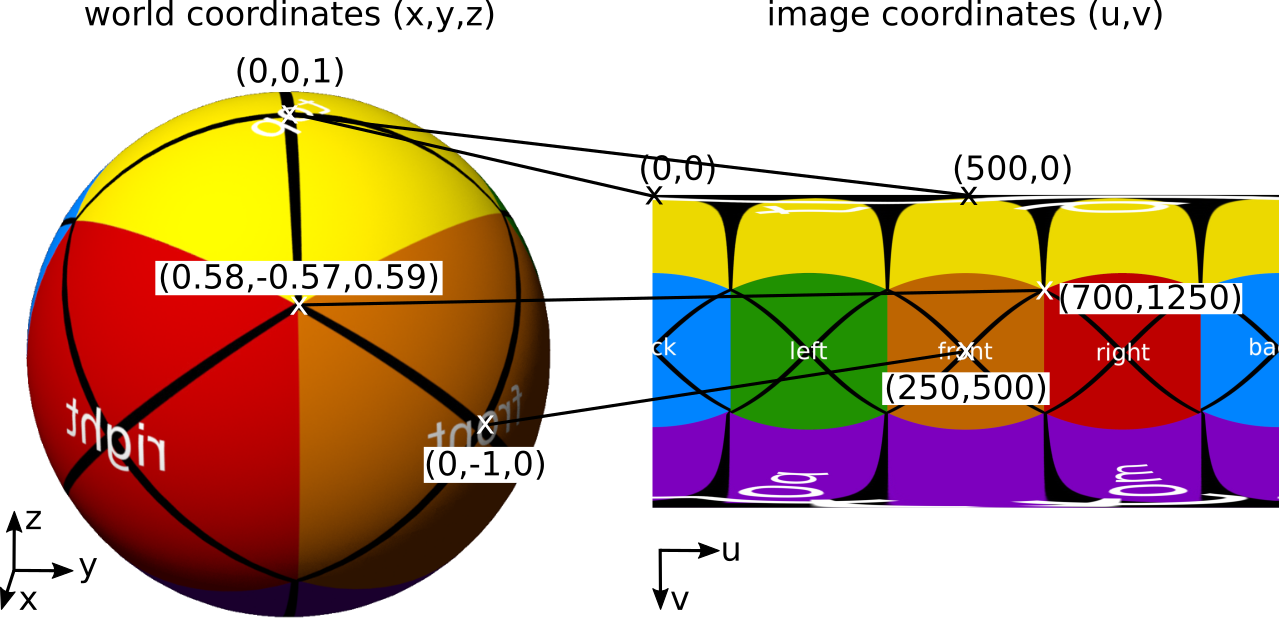
\includegraphics[width=0.8\textwidth]{02/uv_mapping.png}
		\caption[UV mapping example]{UV mapping example using an equirectangular image}
		\label{fig:uv_mapping}
\end{figure}

In the case of 360\degree images, the first step after capture is to convert the captured color values to a a planar image for storage and viewing. There are a number of common different mappings for this task from which to choose from, depending on the application.

\subsubsection{Mappings for Planar Representation of 360\degree Images \cite{hdrbook}}\label{subsec:projections}
The most common mappings for 360\degree images are the \emph{cube map}, the \emph{ideal mirrored sphere}, the \emph{angular map},  and the \emph{equirectangular map} \cite{hdrbook}. The image data can be projected with any of these mappings without data loss.\todo{not 100\% sure that this is true}

\paragraph{Cube Map}
The cube map is a mapping that splits the data into six separate square views, one in each direction (top, front, left, right, back, bottom). This is the equivalent of capturing the surroundings with six different cameras with a field of view of 90\degree each, and then stitching the resulting images into a shape that can be ``folded'' into a cube (see Figure~\ref{fig:cubemap-intro}), which also gives this mapping its name.

Due to the projection of a spherical surface to a plane, there is some distortion towards the edges of each face. However, this distortion is comparable to the distortion at the edges of a regular, planar image, which is a significant advantage compared to other mappings. The disadvantage is that each face is projected separately, which leads to directional discontinuities at the many seams. This type of mapping is often used to simulate complex environments in 3D scenes (e.g. for game or animation graphics), as it is easy to use and reduces render time significantly compared to a 3D model of the same environment.
\cite{hdrbook}

\paragraph{Ideal Mirrored Sphere}
The ideal mirrored sphere is a mapping to a circle within a square. It represents how the surroundings would be reflected by a perfect mirrored sphere photographed by an orthographic camera, given the size of the sphere was considerably smaller than the distance to the surroundings. This mapping, like all the mappings presented here, shows the complete surroundings, albeit very distorted toward the edges. Figure~\ref{fig:sphere-intro}b shows where each direction is mapped and the extent of the distortion. It is clear that the farther away from the ``front'' area, the more distorted the mirrored sphere mapping is. The ideal mirrored sphere mapping can be used for calculating average illumination color for high dynamic range calculations, however, the type of distortion at the edges can cause problems with sampling, which is why the angular map mapping tends to be preferred.
\cite{hdrbook}

\paragraph{Angular Map}
At first sight, the angular map seems very similar to the ideal mirrored sphere. It also maps to a circle within a square, however it samples the input in such a way that the back of the image is allotted more space and is less distorted than the mirrored sphere (see Figure~\ref{fig:angular-intro}). This mapping is also used for high dynamic range calculations.

\paragraph{Equirectangular Map}
The equirectangular, or latitude-longitude (latlong) mapping is a common type of mapping in cartography. The data is mapped to a rectangular image space, in which the width is twice the height. The azimuth (around the circumference) of the world coordinates is mapped to the map's horizontal coordinate and the elevation to the vertical coordinate. The main problem of this representation is well known in cartography: The distortion increases significantly towards the poles, as can be seen in Figure~\ref{fig:latlong-intro}. Otherwise, this mapping is convenient as it has very few seams and all pixels are valid (i.e. no ``black'' areas). It is used as a storage format for 360\degree images.

\paragraph*{}
All of these projections are static, showing the entirety of the 360\degree image at once. It is also possible to view 360\degree images interactively. In this case the field of view tends to be limited, so only a certain part of the image needs to be projected: the part of the image the viewer is ``facing'' virtually. Once the viewing direction has been determined, the projection can be calculated such that the center of the image has minimal distortion. Theoretically, any of the above projections could be used for this. 

\begin{figure}
\centering
    \begin{subfigure}[t]{0.5\textwidth}            
            \centering
            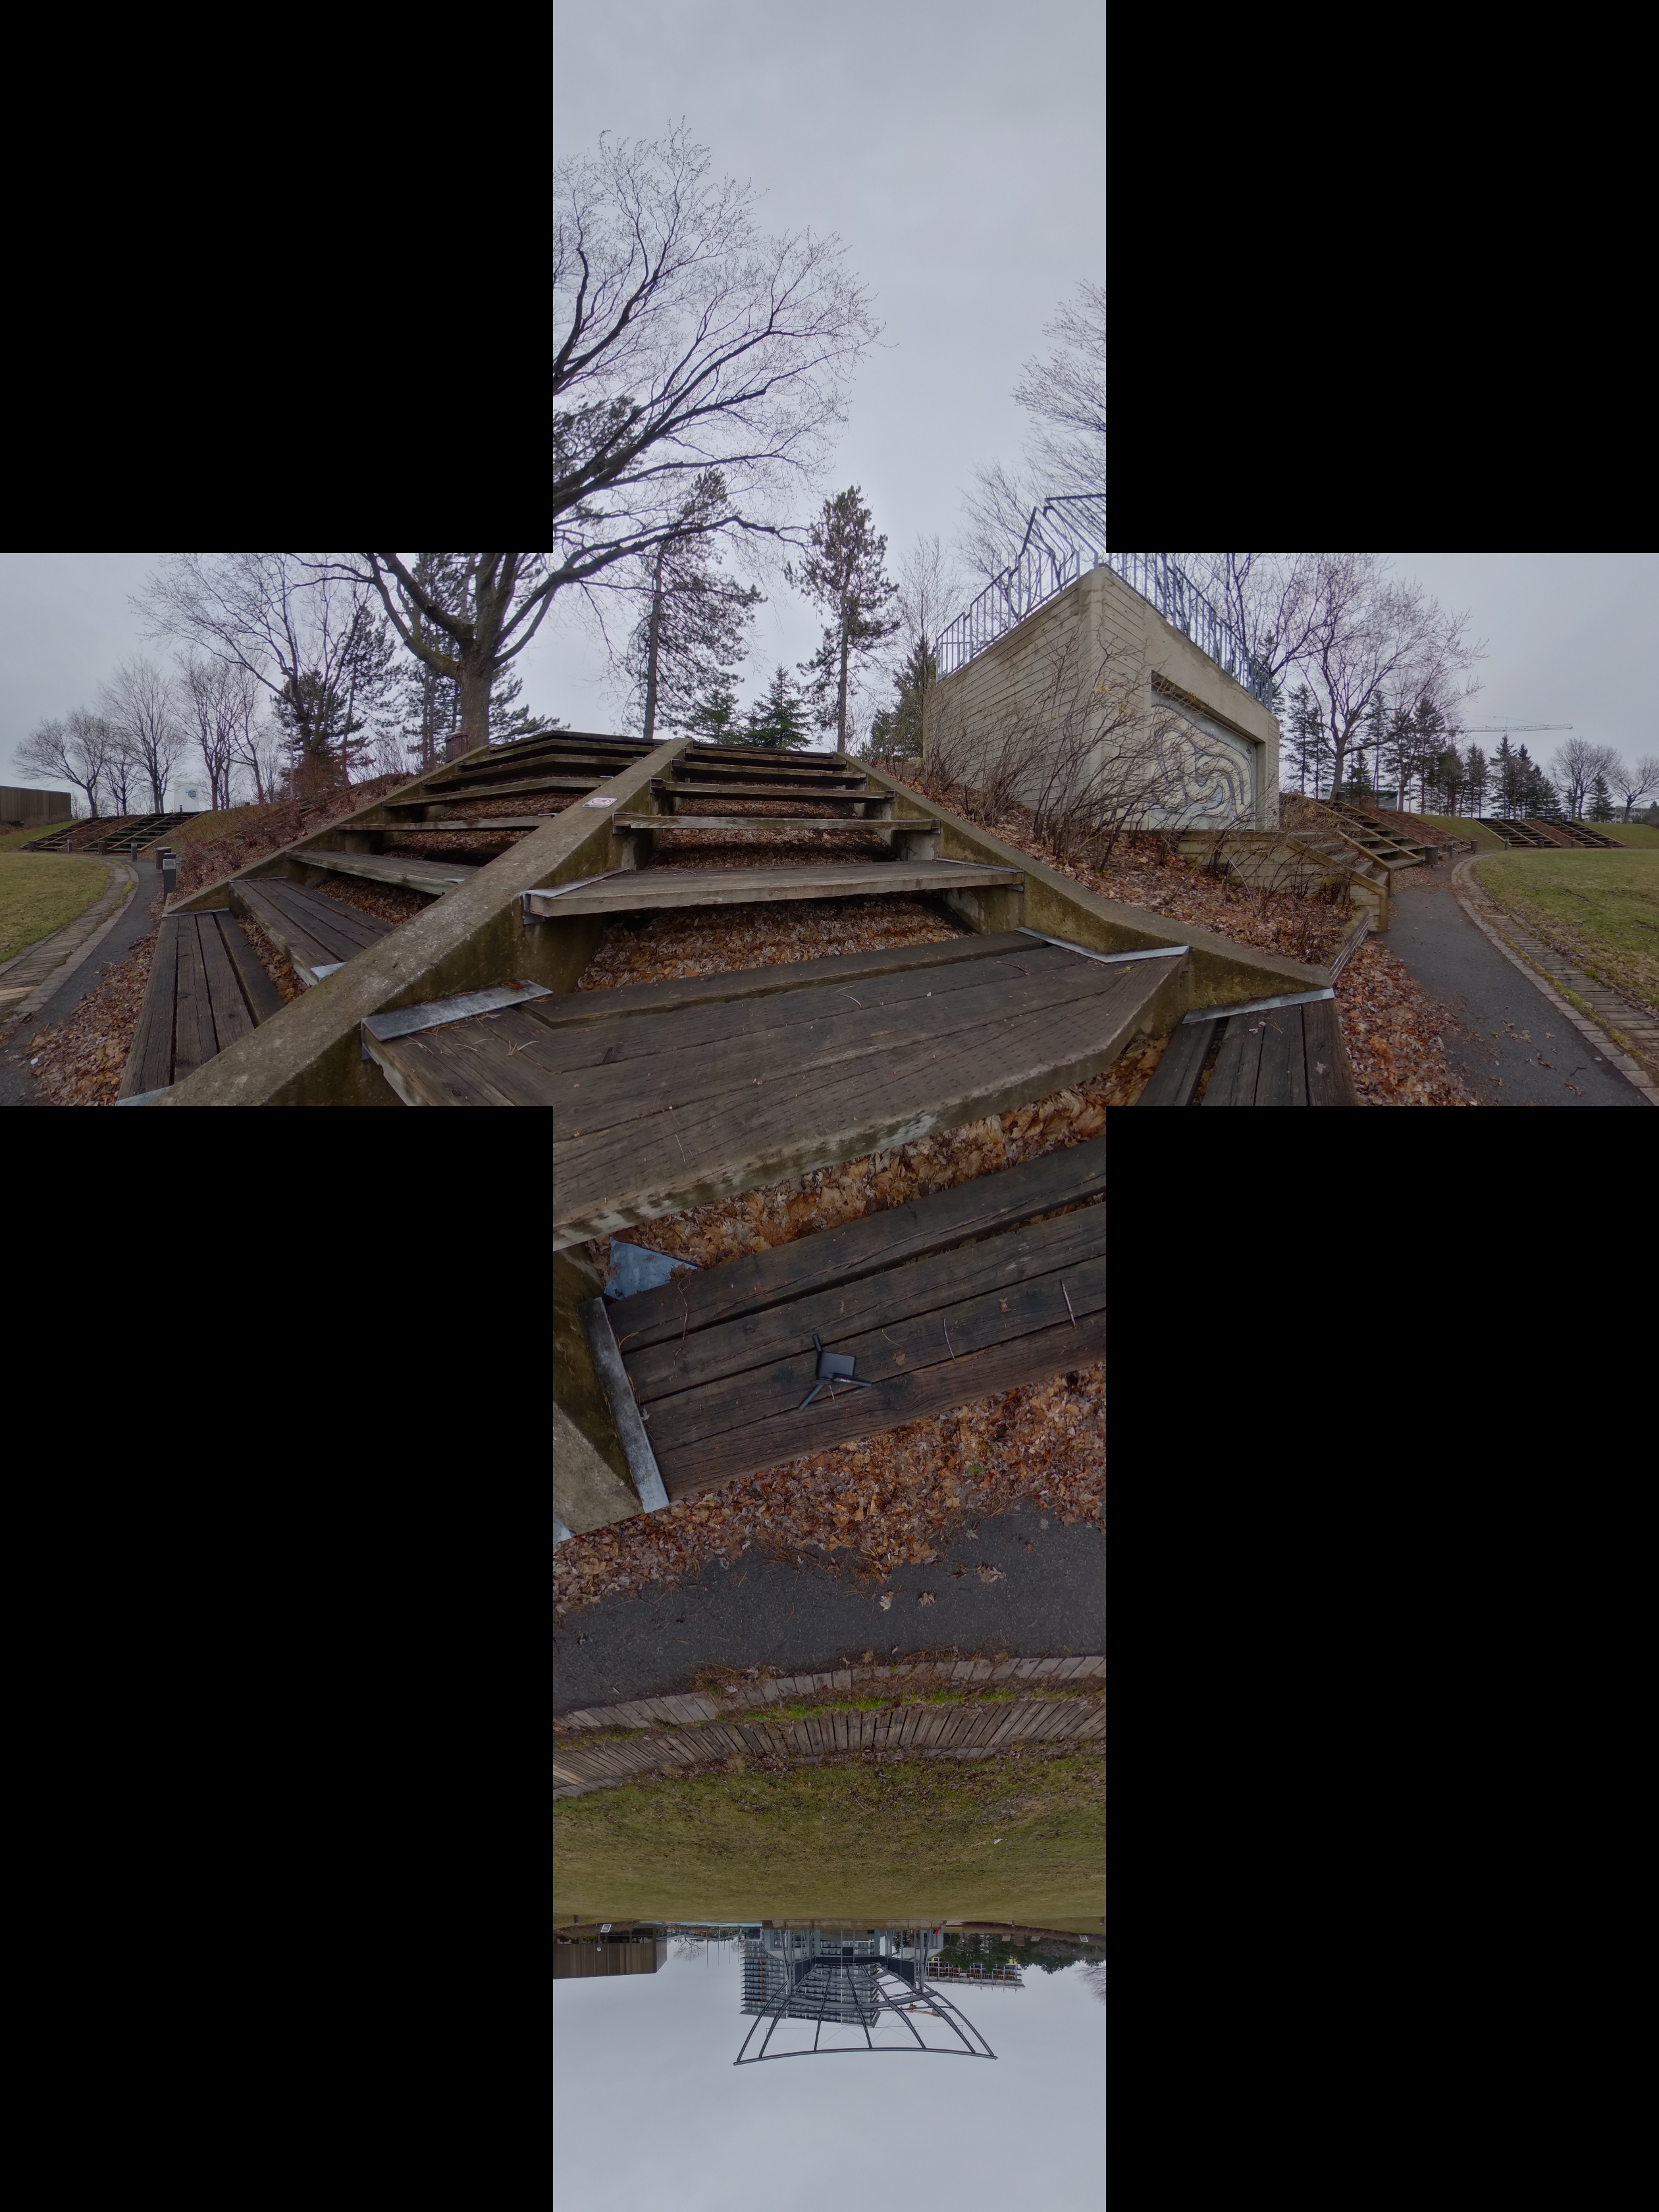
\includegraphics[width=0.5\textwidth]{02/mapping_cube_photo.jpg}
            \caption{360\degree image as a cube map}
    \end{subfigure}%
     %add desired spacing between images, e. g. ~, \quad, \qquad etc.
      %(or a blank line to force the subfigure onto a new line)
    \begin{subfigure}[t]{0.5\textwidth}
            \centering
            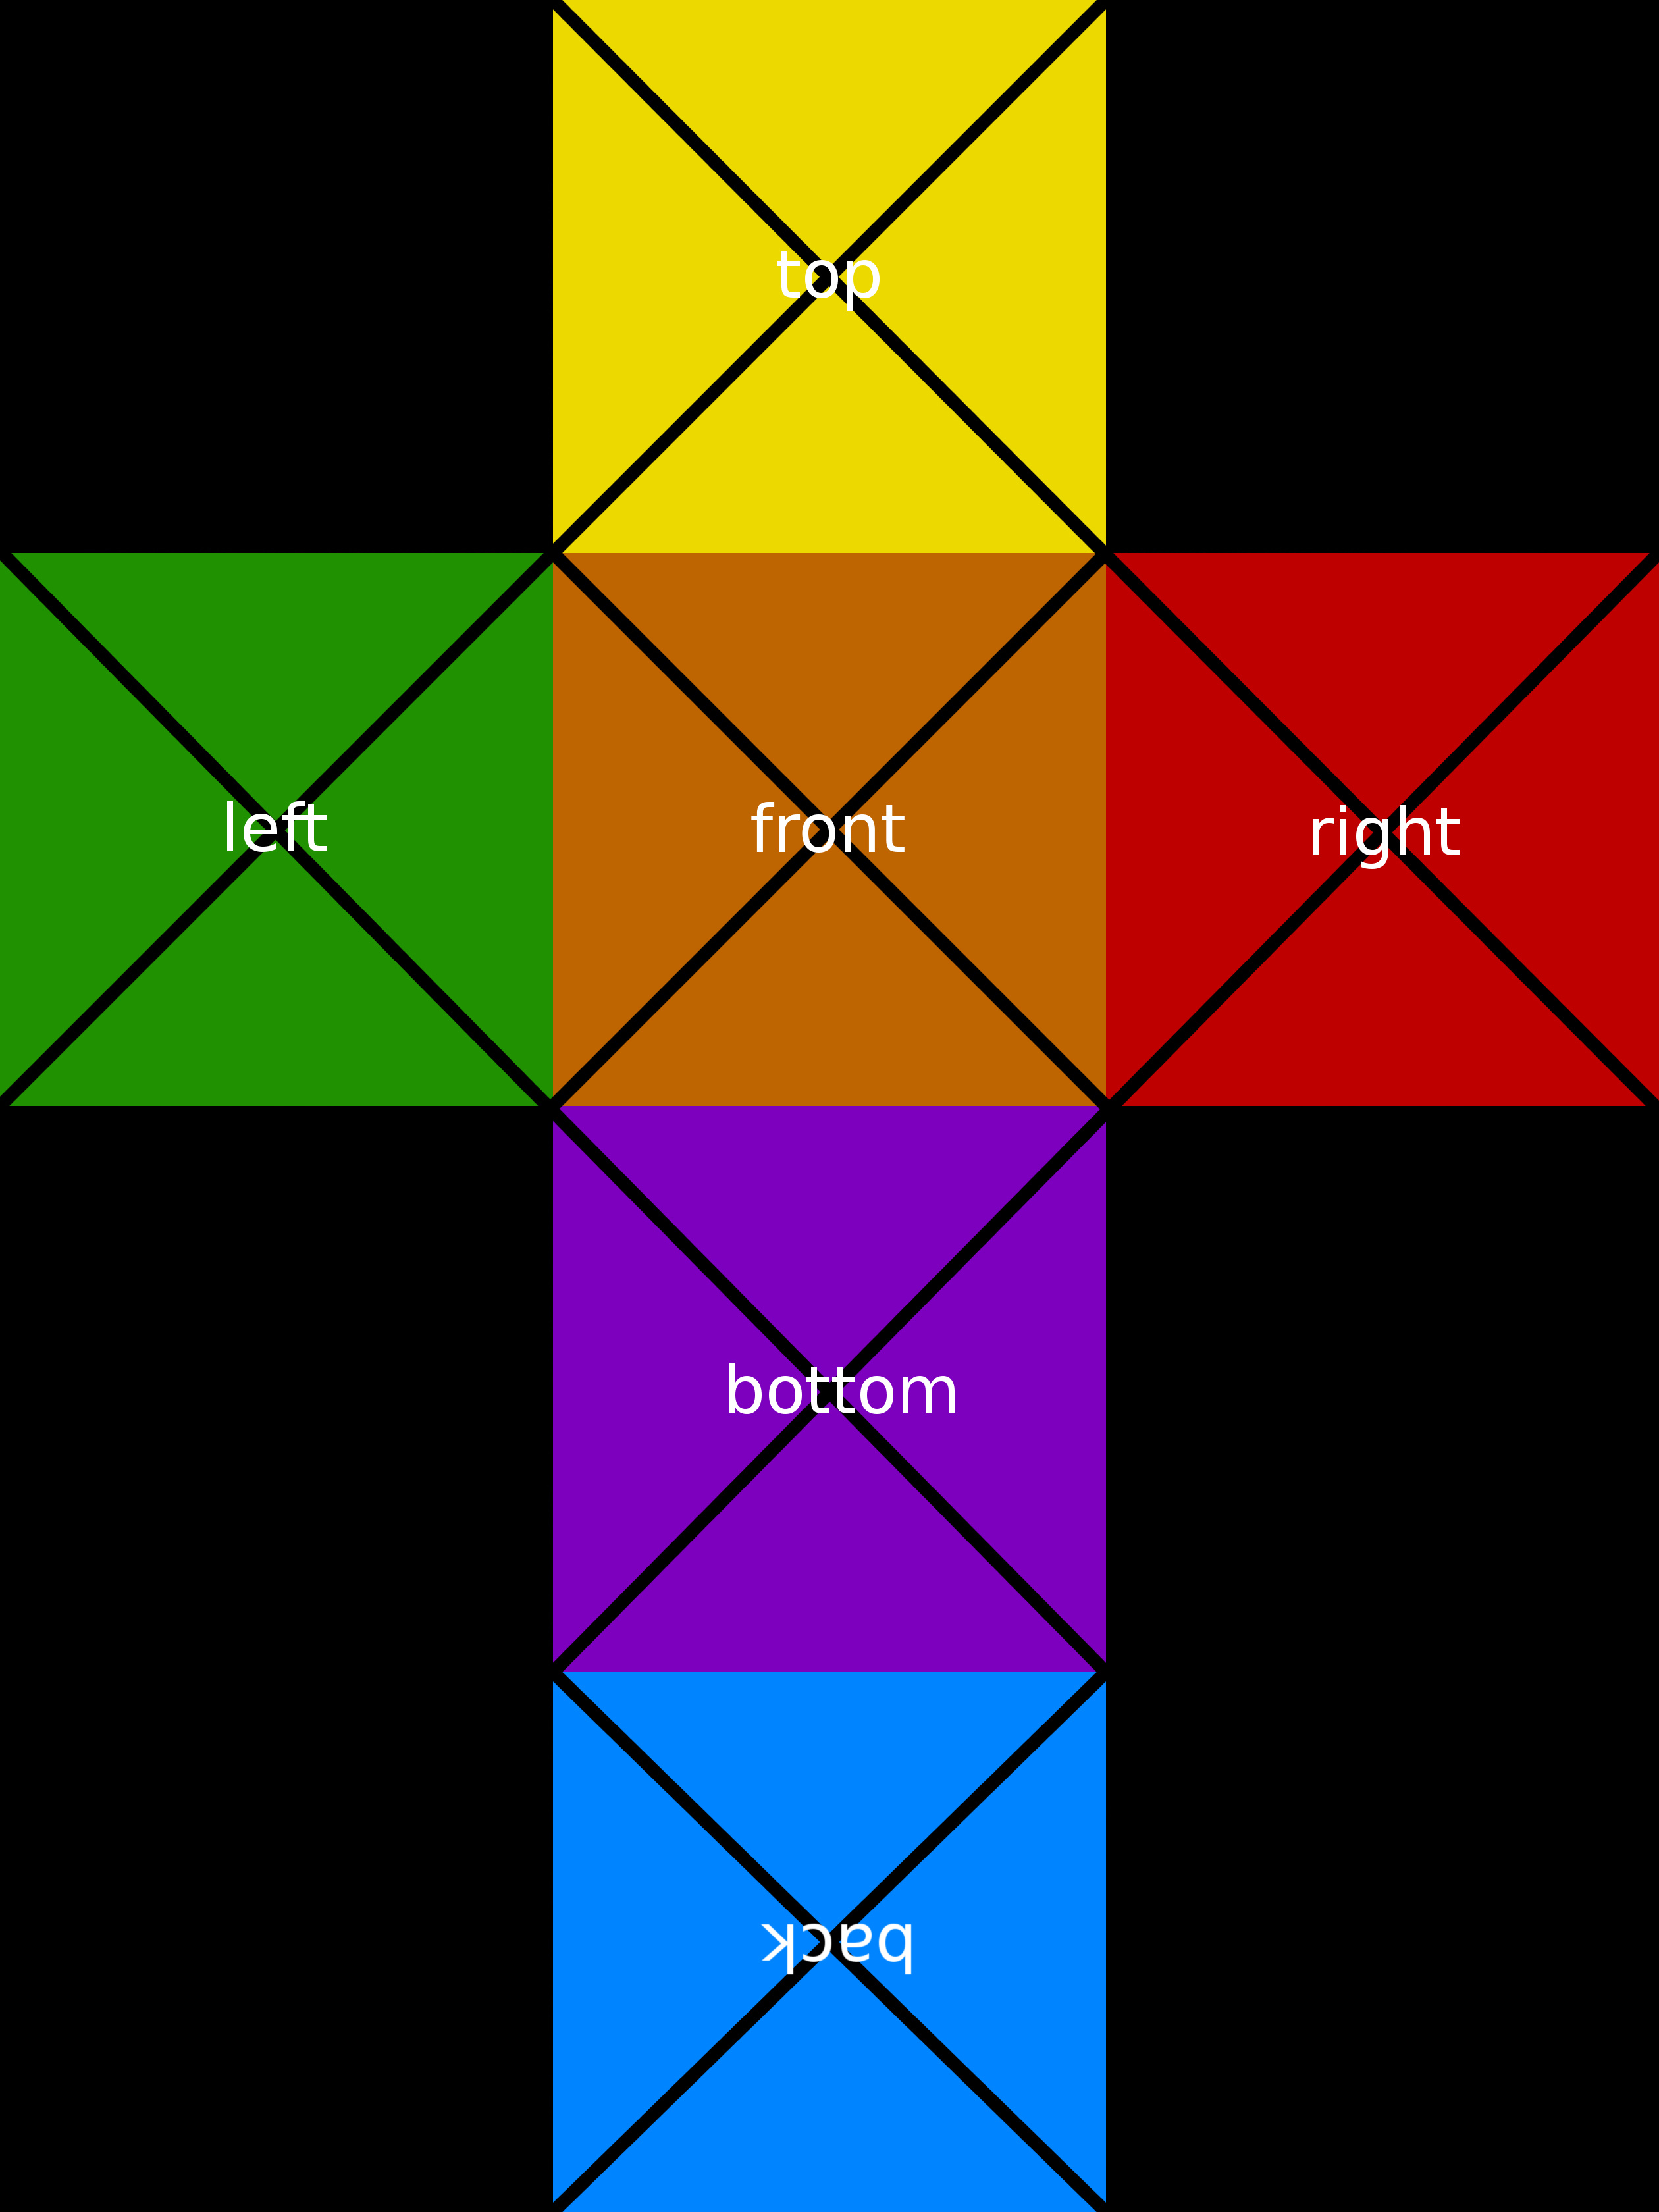
\includegraphics[width=0.5\textwidth]{02/mapping_cube.jpg}
            \caption{Distortion visualization}
    \end{subfigure}
    \caption[Cube map mapping]{The cube map mapping}\label{fig:cubemap-intro}

    \quad
    \begin{subfigure}[t]{0.5\textwidth}
            \centering
            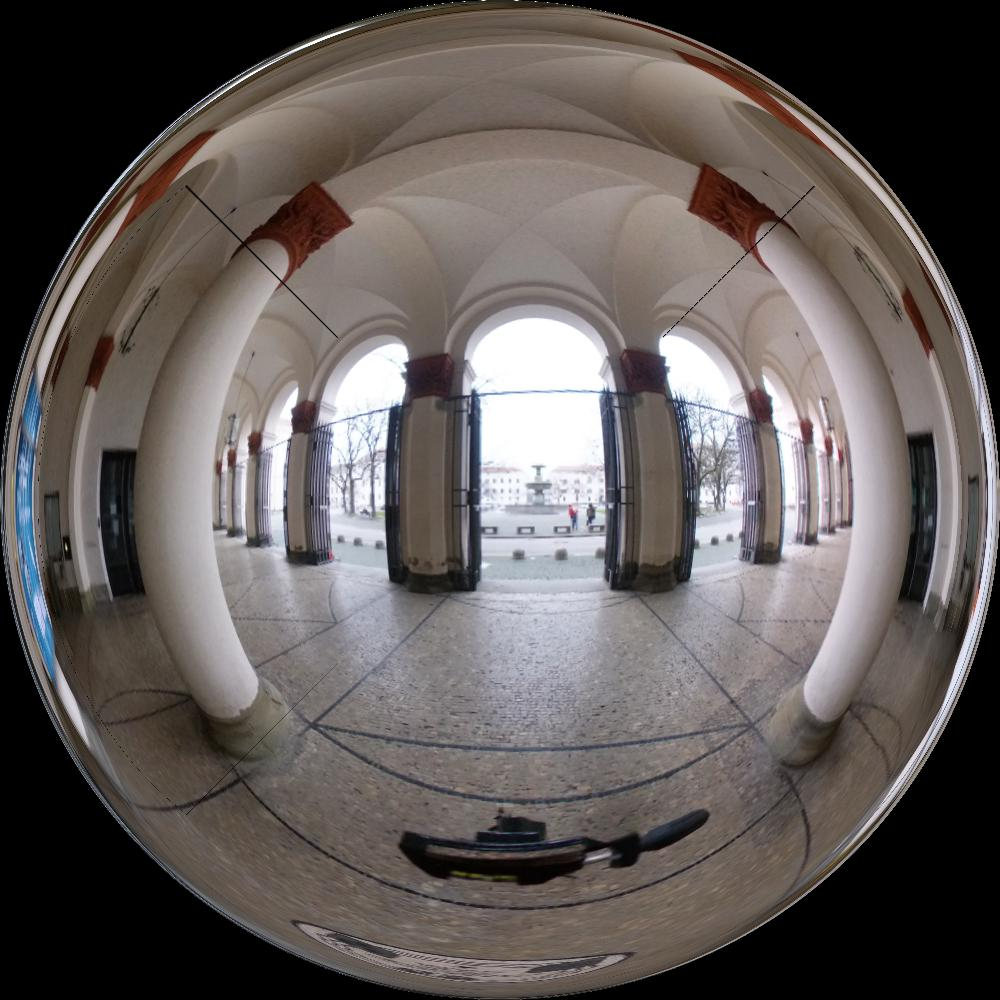
\includegraphics[width=0.5\textwidth]{02/mapping_sphere_photo.jpg}
            \caption{360\degree image as a mirrored sphere mapping}
    \end{subfigure}%
     %add desired spacing between images, e. g. ~, \quad, \qquad etc.
      %(or a blank line to force the subfigure onto a new line)
    \begin{subfigure}[t]{0.5\textwidth}
            \centering
            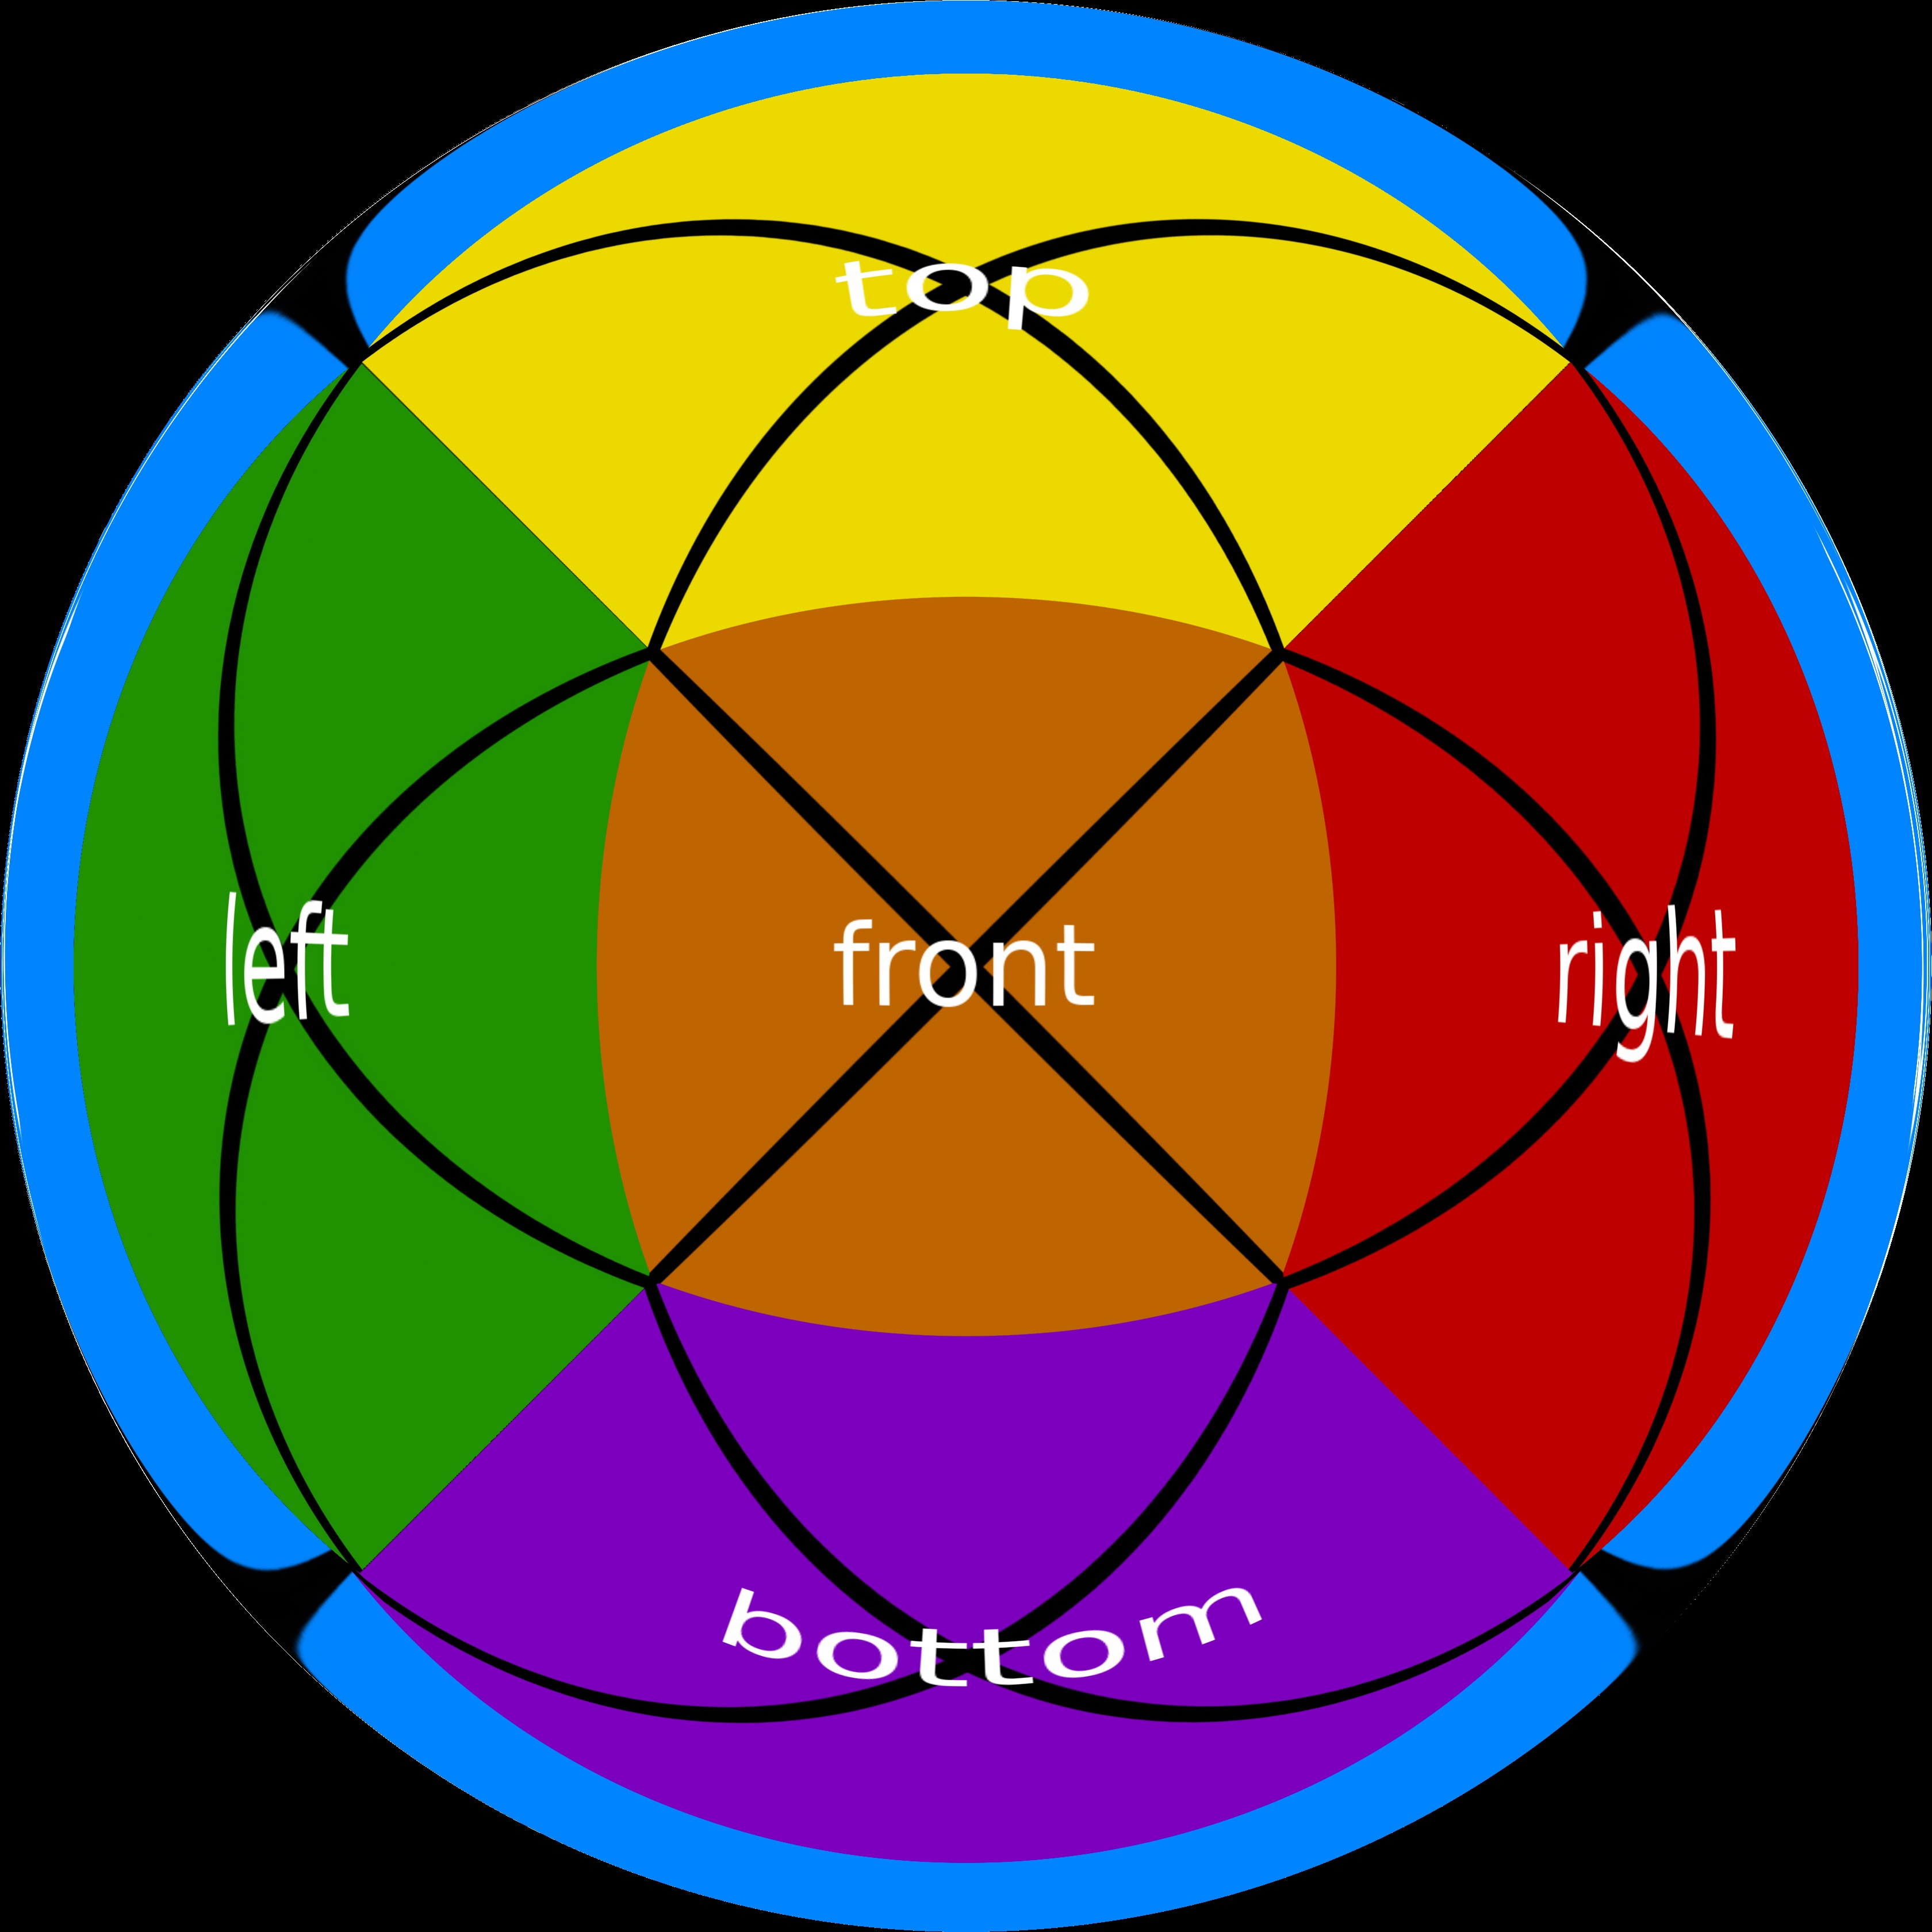
\includegraphics[width=0.5\textwidth]{02/mapping_sphere.jpg}
            \caption{Distortion visualization}
    \end{subfigure}
    \caption[Mirrored sphere mapping]{The mirrored sphere mapping}\label{fig:sphere-intro}

    \quad
    \begin{subfigure}[t]{0.5\textwidth}            
            \centering
            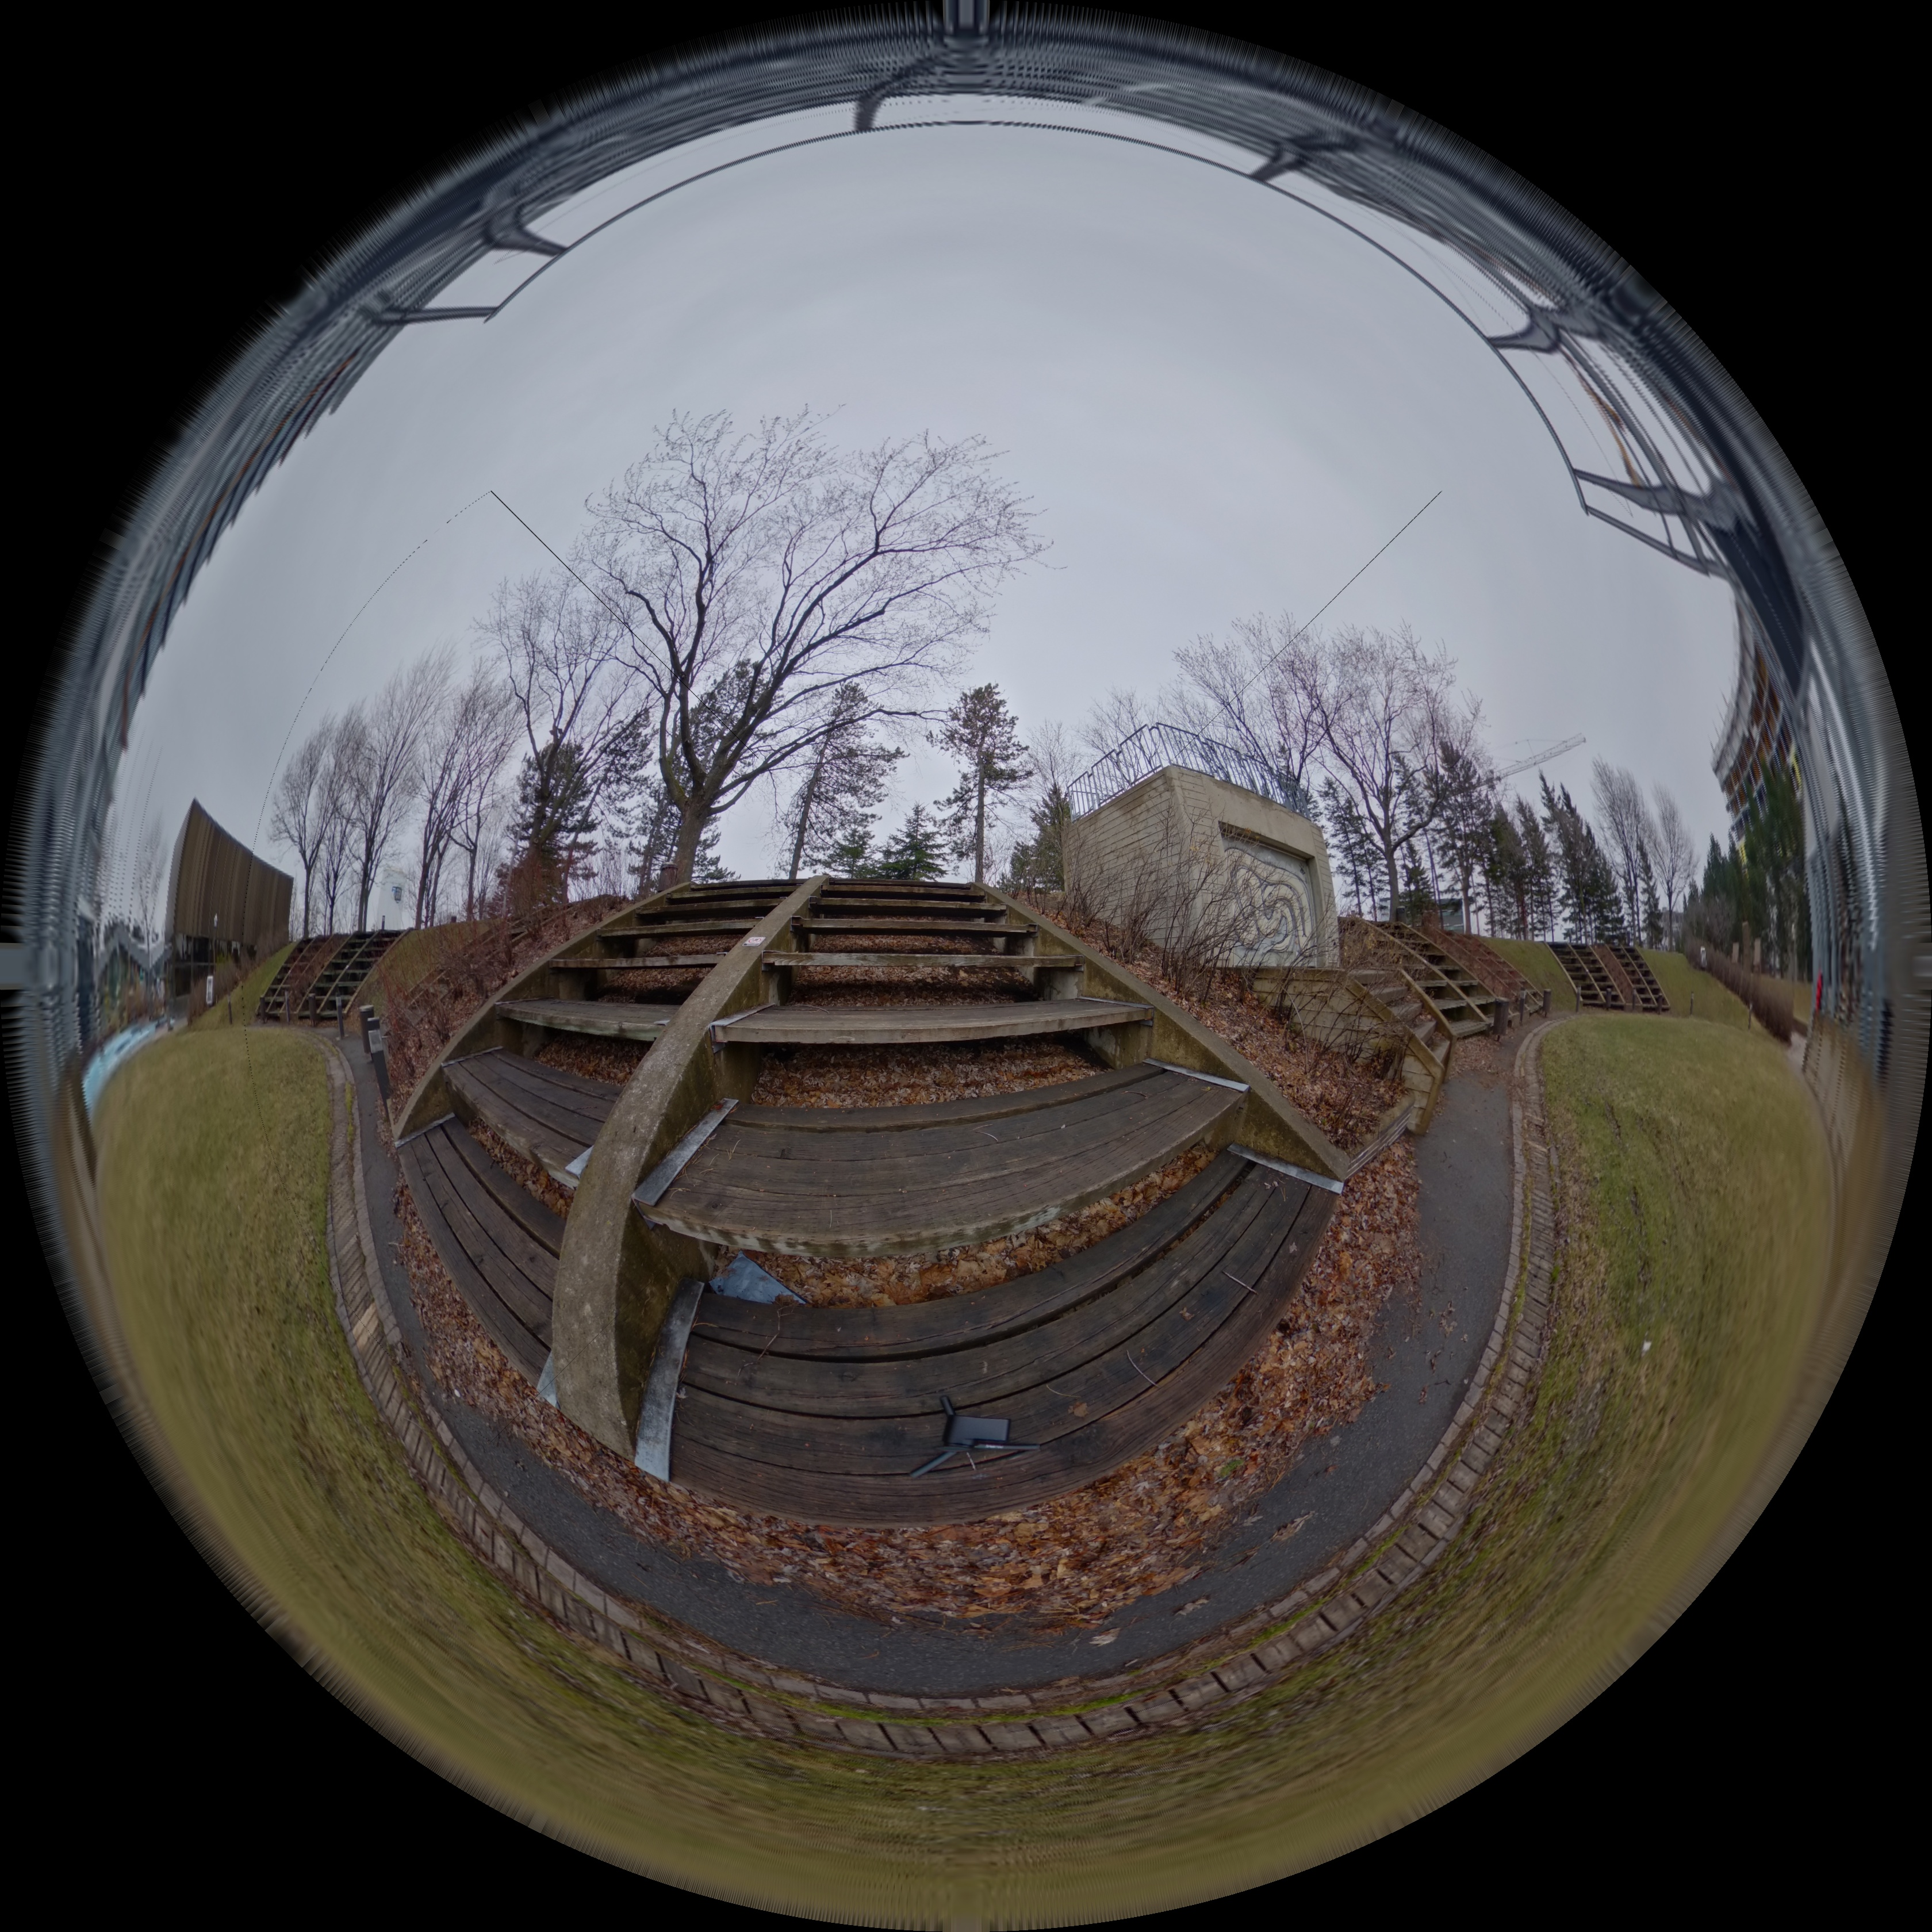
\includegraphics[width=0.5\textwidth]{02/mapping_angular_photo.jpg}
            \caption{360\degree image as an angular mapping}
    \end{subfigure}%
     %add desired spacing between images, e. g. ~, \quad, \qquad etc.
      %(or a blank line to force the subfigure onto a new line)
    \begin{subfigure}[t]{0.5\textwidth}
            \centering
            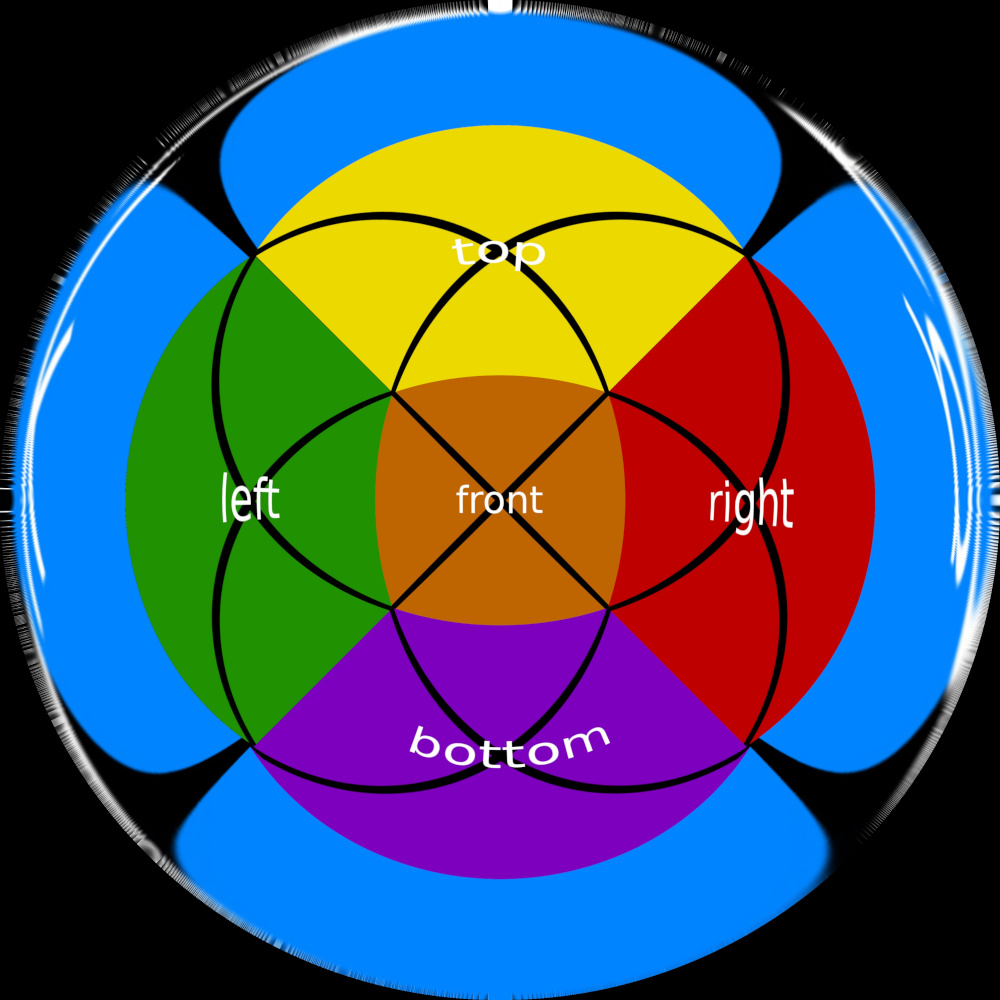
\includegraphics[width=0.5\textwidth]{02/mapping_angular.jpg}
            \caption{Distortion visualization}
    \end{subfigure}
    \caption[Angular mapping]{The angular mapping}\label{fig:angular-intro}

    \quad
    \begin{subfigure}[t]{0.5\textwidth} 
            \centering
            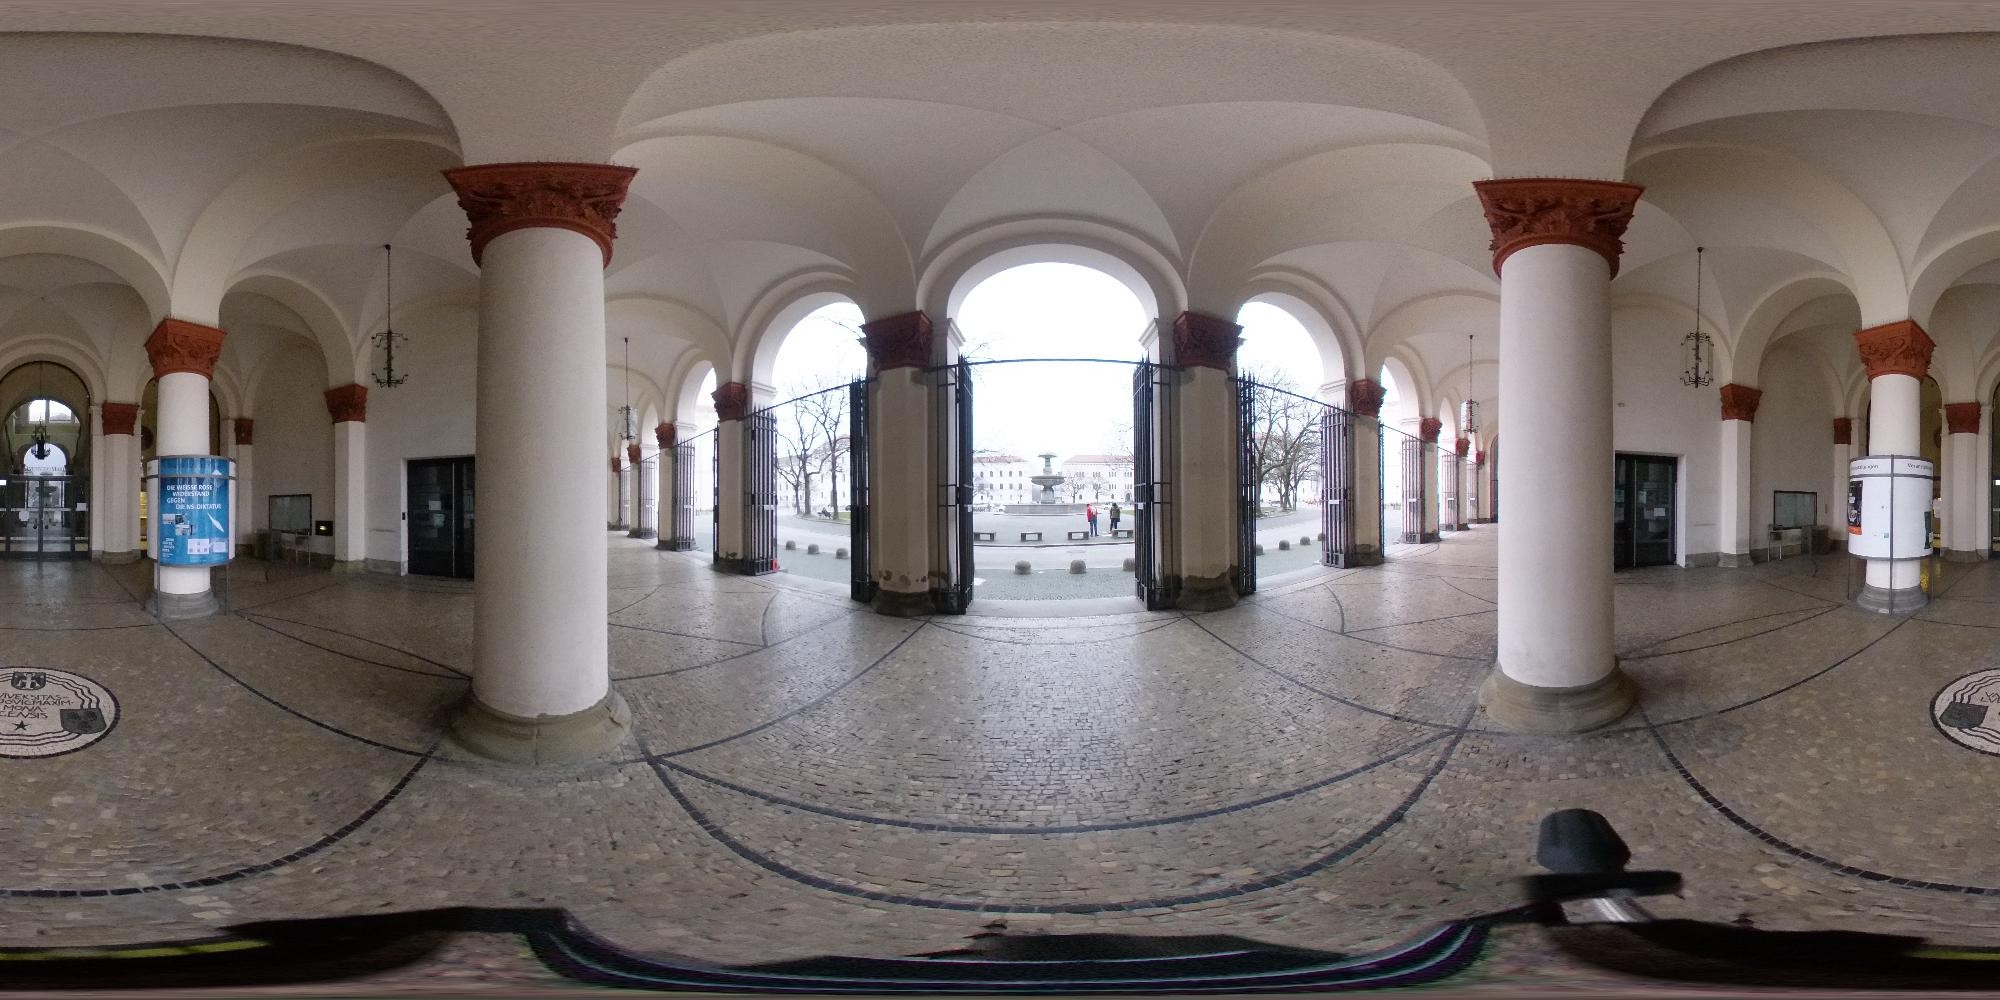
\includegraphics[width=0.9\textwidth]{02/mapping_latlong_photo.jpg}
            \caption{360\degree image as a latlong mapping}
    \end{subfigure}%
     %add desired spacing between images, e. g. ~, \quad, \qquad etc.
      %(or a blank line to force the subfigure onto a new line)
    \begin{subfigure}[t]{0.5\textwidth}
            \centering
            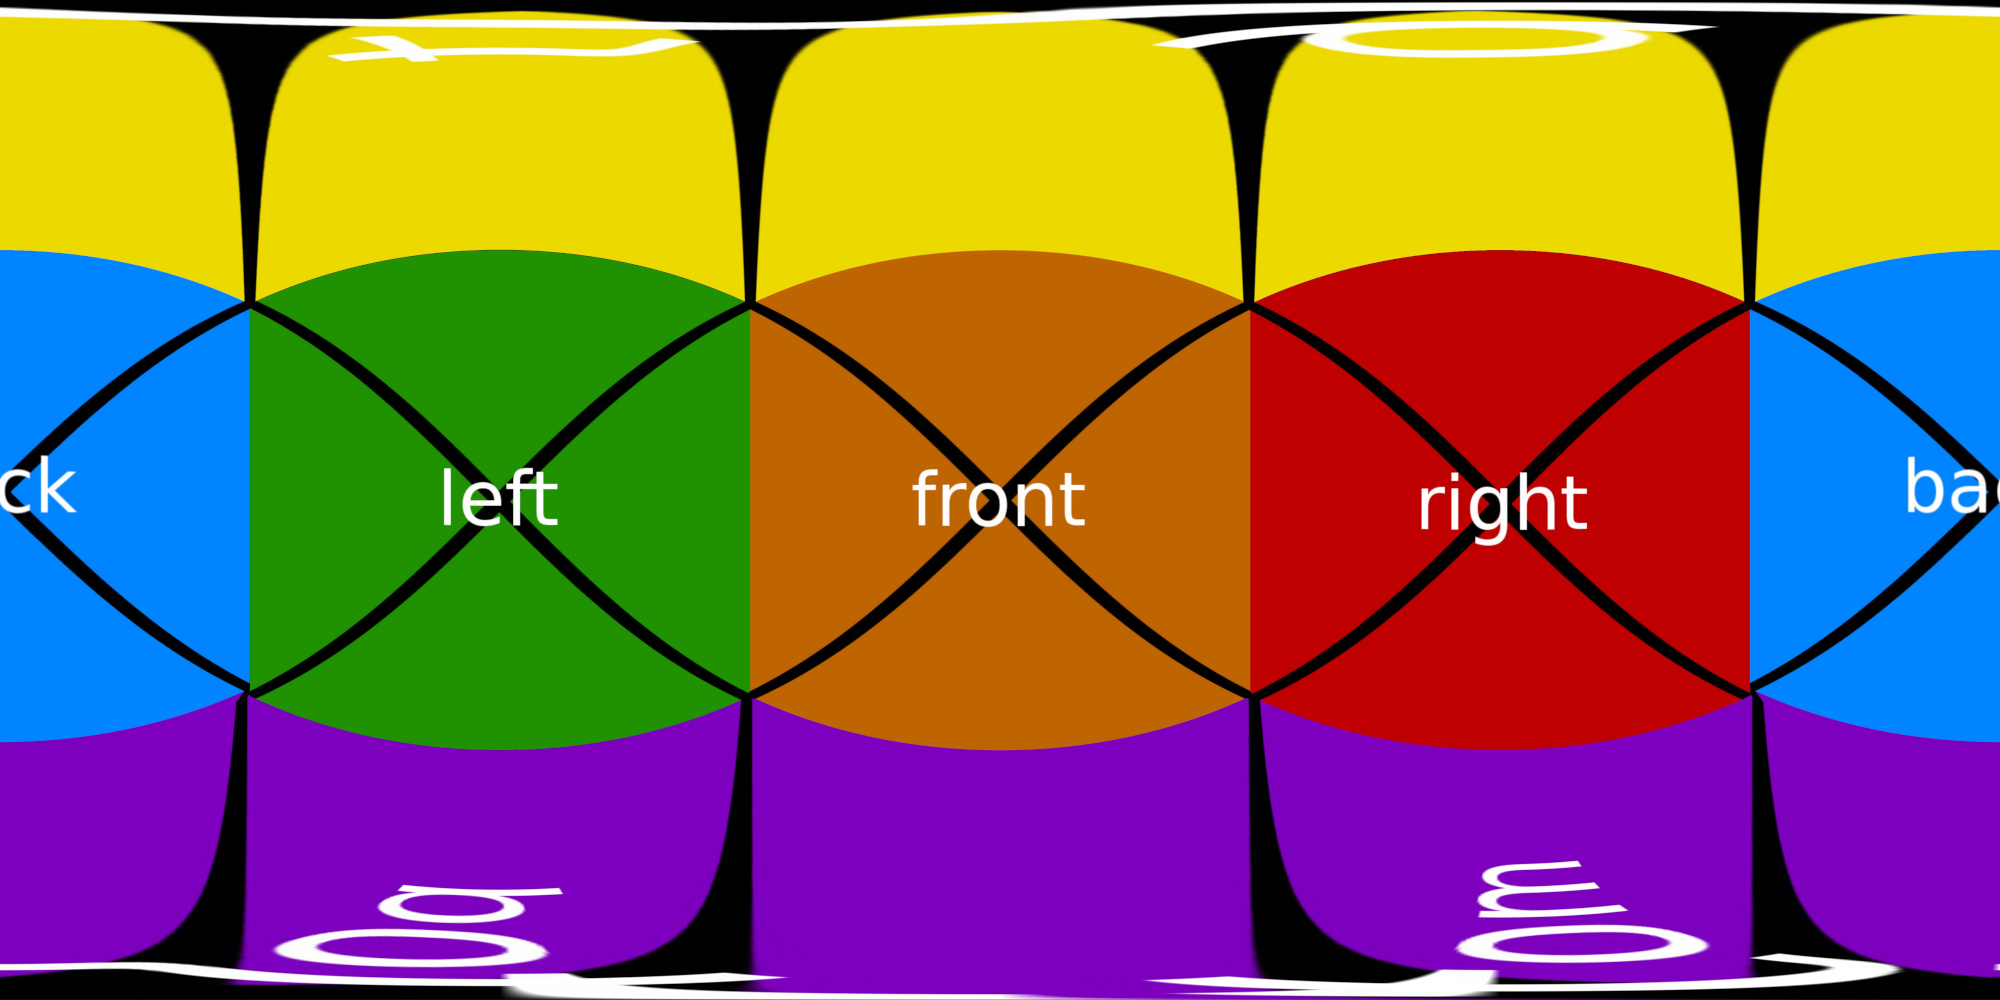
\includegraphics[width=0.9\textwidth]{02/mapping_latlong.jpg}
            \caption{Distortion visualization}
    \end{subfigure}
    \caption[Latlong mapping]{The latlong mapping}\label{fig:latlong-intro}
  \end{figure}
  \footnotetext{Figure~\ref{fig:cubemap-intro}b does not correctly represent the distortion in cube maps. It was chosen as a baseline because cube maps have relatively small distortion compared to other mappings and it visualizes clearly which parts of the image are mapped where.}

\subsection{Optical Flow} \label{subsec:optical_flow}
Optical flow describes the displacement of specific points between two images. It is generally used on consecutive frames of video sequences, for example for semantic segmentation, structure-from-motion, data compression or other applications where information about movement between images is required. To illustrate, Figure~\ref{fig:of_example_bike} shows two consecutive frames of a video sequence. On a high level, an optical flow algorithm should recognize that the pixels representing the bicyclist are moving towards the bottom left of the image, and the pixels representing the background are moving to the right (because the camera is panning slightly to the left).

There are two types of optical flow: Sparse optical flow and dense optical flow. Sparse optical flow algorithms calculate the motion of several select points that can be either chosen manually, or by some kind of automatic selection (e.g. based on features). This type of optical flow can be used to track only specific objects in a scene (e.g. the direction and relative velocity of a certain car in traffic).

Dense optical flow algorithms compute the motion of \emph{each pixel} between two images, which yields a more exact result than sparse optical flow. This can be used for more general object tracking (e.g. direction and relative velocity of complete surroundings in traffic), to estimate 3D geometry (in structure-from-motion algorithms), or to identify static sections of the image for video compression. Dense optical flow can also be used for image synthesis, such as in Richardt et al's Megastereo \cite{megastereo} described in Section~\ref{subsec:megastereo}, which is also the basis of the flow-based interpolation presented in this thesis.

There are a number of optical flow algorithms, ranging from methods using parametrization, or regularization \cite{of-survey}, to methods relying on Deep Learning \cite{of-deep}. Although these algorithms differ greatly in approach, they have in common the type of result, which is a vector field. For dense optical flow, this vector field contains a vector for each pixel, describing the displacement of this pixel between the input images. Sparse optical flow only contains a vector for each pre-chosen point, not for every pixel.

Figure~\ref{fig:of_vis} shows two different visualizations of the vector field calculated by the dense optical flow algorithm by Farneb\"ack \cite{farneback} between the frames in Figure~\ref{fig:of_example_bike}. Figure~\ref{fig:of_vis}a is a color-based visualization: the hue encodes the vector direction, the saturation encodes the vector length for each pixel. Using this visualization, it is possible to roughly distinguish two separately moving areas of the image, which could be used for semantic segmentation. Figure~\ref{fig:of_vis}b shows the pixel displacements with vectors: the origin of the vector is shown by a point and the direction and length of the vector are represented by a line.

These visualizations can help in understanding if and how well an optical flow algorithm is working. Although there are a large number of different algorithms, most of them still struggle with common issues such as occlusions, too-large displacements and intensity changes \cite{of-survey}. Occlusions are problematic, since the displacements between two images may reveal or cover image areas that, as a result, have no correspondence in the previous image. This problem is exacerbated when displacements are very large (e.g. due to fast-moving objects). Large displacements are also problematic by and of themselves, as most algorithms are not designed to handle them. How these limitations affect the use of optical flow for image synthesis will be explored in chapters~\ref{chap:implementation} and \ref{chap:evaluation}.

\begin{figure}
\centering
    \begin{subfigure}[t]{0.5\textwidth}            
            \centering
            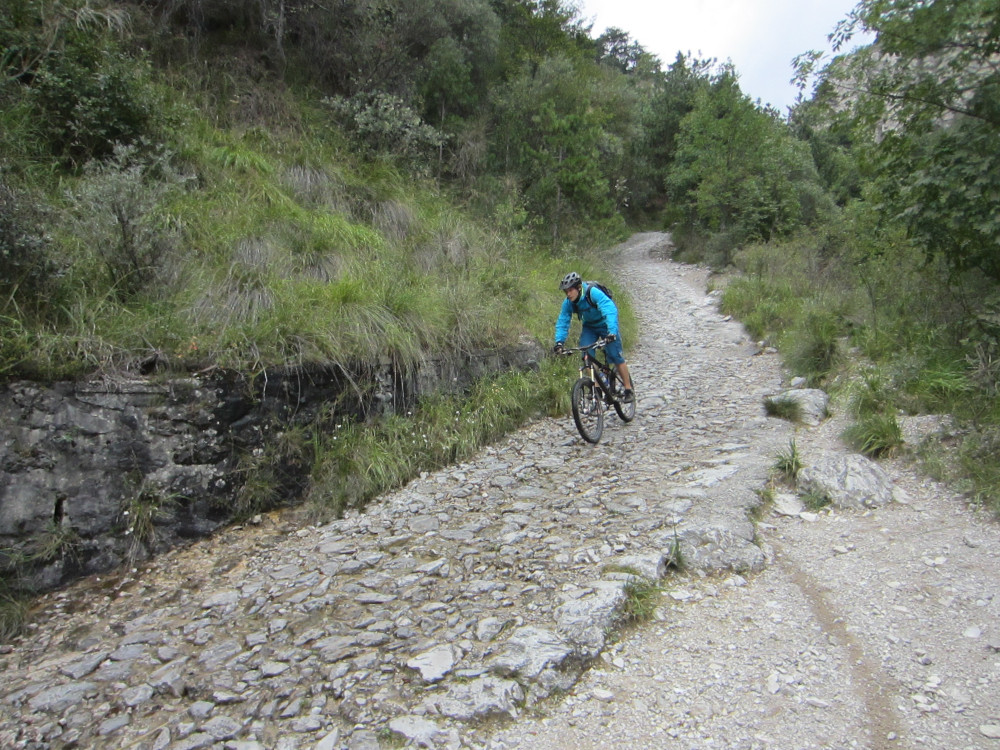
\includegraphics[width=0.9\textwidth]{02/of_example1.jpg}
            \caption{Frame 1}
    \end{subfigure}%
     %add desired spacing between images, e. g. ~, \quad, \qquad etc.
      %(or a blank line to force the subfigure onto a new line)
    \begin{subfigure}[t]{0.5\textwidth}
            \centering
            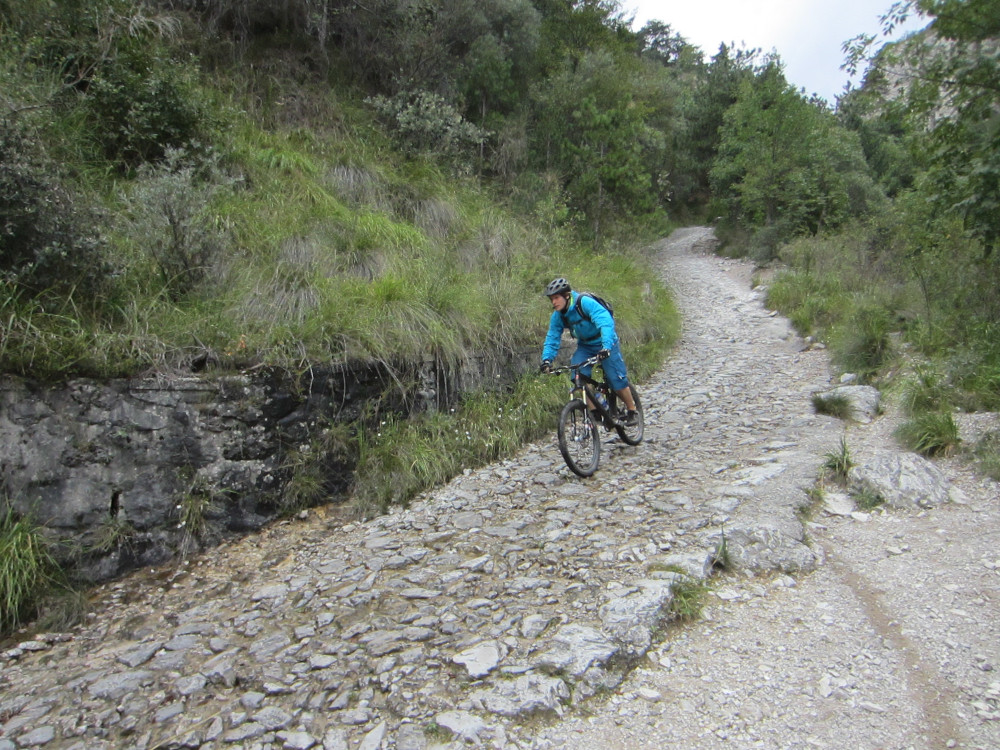
\includegraphics[width=0.9\textwidth]{02/of_example2.jpg}
            \caption{Frame 2}
    \end{subfigure}
    \caption[Optical flow example]{Example frames that optical flow is calculated on}\label{fig:of_example_bike}

    \quad
    \begin{subfigure}[t]{0.5\textwidth}            
            \centering
            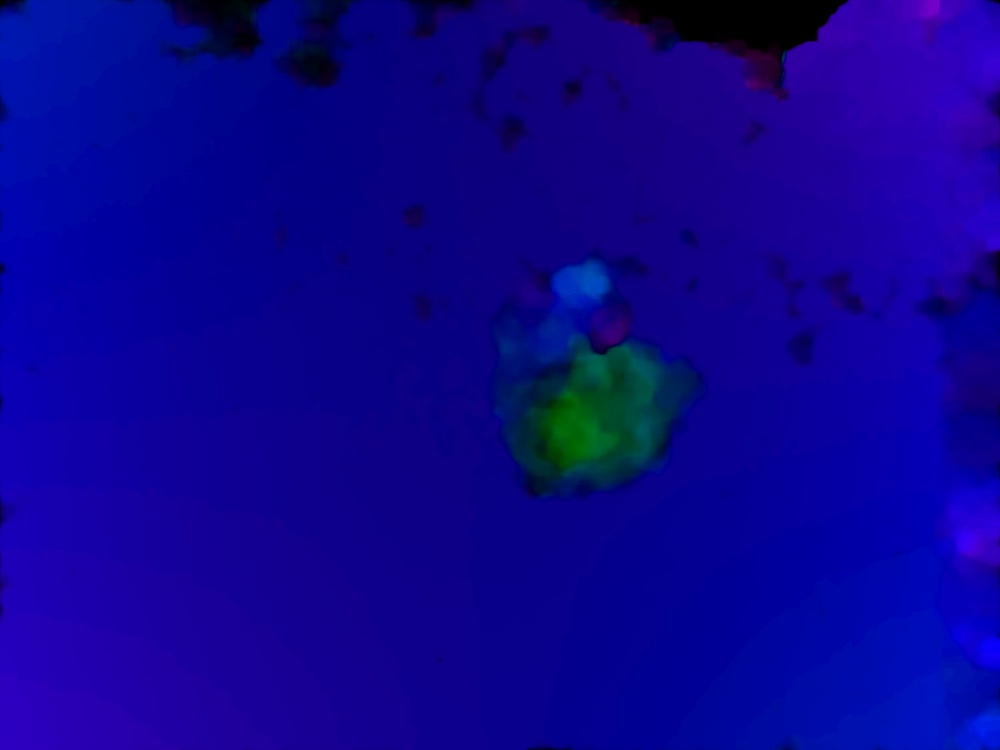
\includegraphics[width=0.9\textwidth]{02/of_vis1.jpg}
            \caption{Visualization of optical flow with color: the hue encodes the vector direction, the saturation encodes the vector length for each pixel.}
    \end{subfigure}%
     %add desired spacing between images, e. g. ~, \quad, \qquad etc.
      %(or a blank line to force the subfigure onto a new line)
    \begin{subfigure}[t]{0.5\textwidth}
            \centering
            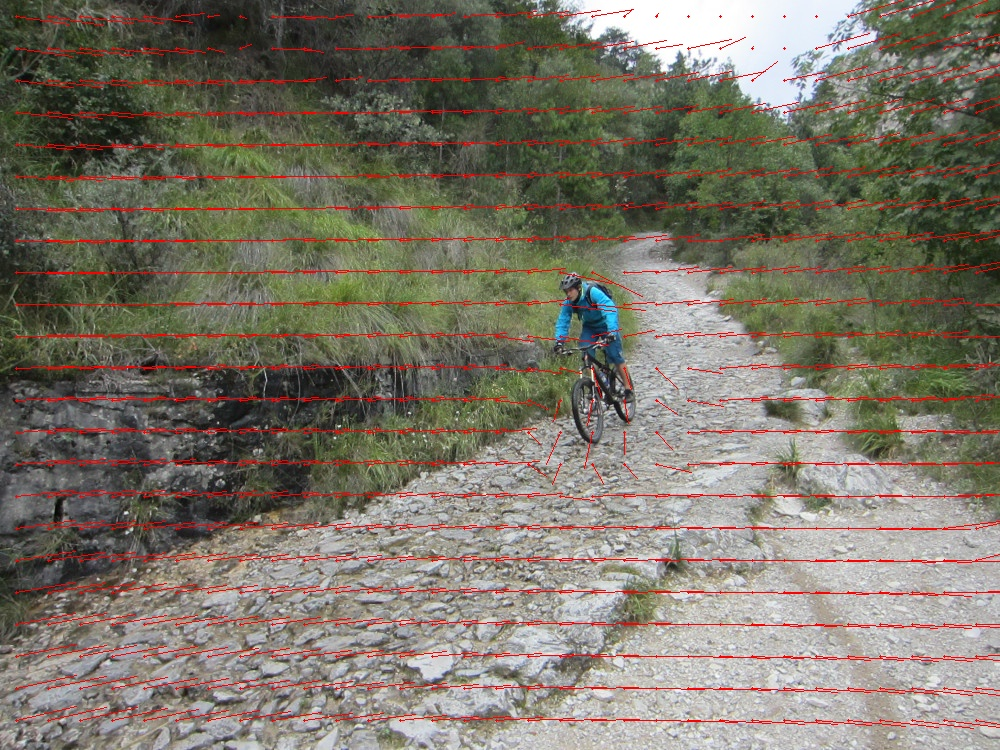
\includegraphics[width=0.9\textwidth]{02/of_vis2.jpg}
            \caption{Visualization of optical flow with vectors: the origin of the vector is shown by a small point (only a limited number of vectors are shown)}
    \end{subfigure}
    \caption[Optical flow visualizations]{Optical flow visualizations}\label{fig:of_vis}
\end{figure}

\section{Related Work}
\begin{comment}
  
Image-based Rendering (IBR) and viewpoint interpolation started gaining interest with the advent of virtual walkthroughs, for example for Apple's QuickTime\textsuperscript{\textregistered} VR, in order to save render time by generating views from images instead of using complex 3D scenes including textures, lights and complex geometric models \cite{quicktime}.

Chen et al., in their survey on image-based rendering \cite{survey2004} use the terms \emph{source description} and \emph{appearance description} to compare these basic rendering techniques: ``Traditional'' rendering techniques use \emph{source description}, i.e. the scene is described by the objects within it, their positions and properties. On the other hand, IBR techniques try to achieve the same goal through \emph{appearance description}. Vision itself has little to do with 3D geometries, it is the processing of a dense set of light rays by the brain which are captured through the eye. This process can also be synthesized by a capture device like a camera. So, instead of trying to describe the scene through the objects it contains, IBR rendering techniques try to model the \emph{light rays} that reach the viewer. 

A theoretical model for \emph{appearance description} was developed by Adelson et al.\ \cite{Adelson91}: the \emph{plenoptic function} (Equation~\ref{eq:plenoptic}). The plenoptic function is a 7D function that describes the observable light at every point in space $V_x$, $V_y$, $V_z$, from every direction $\theta$, $\varphi$, at every wavelength $\lambda$, at every possible point in time $t$.

\begin{equation}
  \label{eq:plenoptic}
  P = P(\theta, \varphi, \lambda, t, V_x, V_y, V_z)
\end{equation}

In practice, it is unfeasible, if not impossible, to cover all dimensions of this function, as this would require a capture device at every location, at every point in time, capturing light rays coming from every direction. However, by making assumptions, IBR techniques try to reconstruct simplified versions of the plenoptic function. Depending on which assumptions are made and how the surroundings are sampled, varying requirements are met and different results are achieved.

Chen et al.\ summarize these different types of assumptions in their survey \cite{survey2004} and categorize different techniques by their use of these assumptions. The first 

Shum et al.\ \cite{survey2000} break different image-based rendering approaches down by categorizing how much geometry is used.  

Many of these approaches however, do use some geometry information in order to recalculate image points. The scene geometry is hereby either meticulously recorded at the time of the image capture, as with Kanade et al's 3D Dome \cite{geometry97}, or inferred from the image data alone, 

The approach presented in this thesis is \emph{pixel-based}, i.e. using no geometry information, so the following section will first outline research aiming to synthesize viewpoints with the use of little to no geometry. Since the majority of pixel-based rendering research uses planar images, the second part will focus on research using 360\degree images, including approaches using geometry.

\begin{itemize}
  \item type of warping: uv mapping, warping based on triangulation and homography
  \item image representation: cube, planar, sphere
  \item constraints? color / angle / \ldots
  \item geometry? sparse, dense, none
  \item correspondences needed? sparse, dense, none
  \item type of input: planar, 360, 180 pano
  \item type of output: planar, 360, 180 pano
\end{itemize}

\subsection{Image Synthesis without 3D Geometry for Planar Images}

\end{comment}
\subsubsection{Megastereo \label{subsec:megastereo}}
\begin{comment}
correspondences needed: dense, geometry: none, constraints: angle?, image rep: planar, type of warping: none, because planar
Richardt et al.\ \cite{megastereo} use a combination of image stitching and their own optical flow-based blending algorithm in order to create high resolution stereo panoramas from a set of planar images captured on a radius. The goal is to synthesize stereoscopic viewpoints (an image for the left and right eye, each) from the captured monoscopic images. After transforming the images so that they all have scene-independent orientation and minimal distortion, strips of the captured images are extracted for each ``eye'' based on the best matching image ray (Figure~\ref{fig:megastereo-figure}a and b). In cases where there is no perfect ray correspondence, the ray with the smallest deviation angle can be chosen, however, this can lead to artefacts as illustrated in Figure~\ref{fig:megastereo-figure}c. In order to mitigate these artefacts, Richardt et al.\ introduce a blending algorithm based on optical flow: 

In order to blend two images, they take the two closest viewpoints $I_K$ and $I_L$ and interpolate $\widetilde{I_M}$ using the optical flow vectors $F_{k\rightarrow l}$ and $F_{l\rightarrow k}$.  The corresponding strip is then taken from this new viewpoint which contains the matching ray (Figure~\ref{fig:megastereo-figure}d).

\begin{figure}[]
\centering
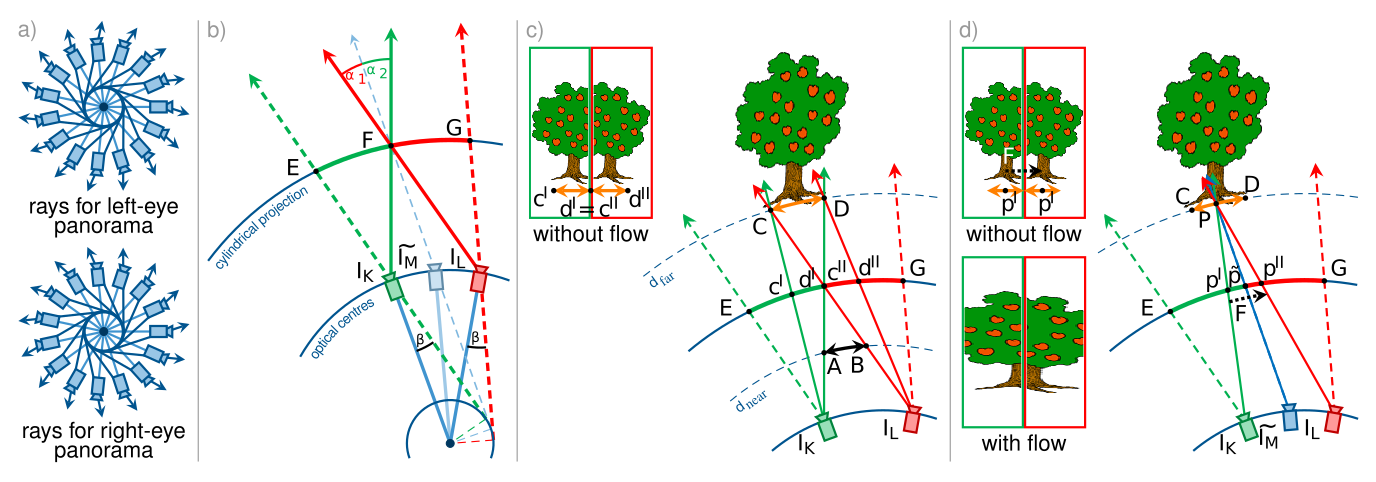
\includegraphics[width=1\textwidth]{02/megastereo-figure.png}
\caption[Flow-based blending in Megastereo]{(a) Illustration of rays required for creating a stereoscopic panorama and (b) deviation angle $\beta$. (c) Duplication and truncation artefacts caused by the aliasing. (d) Flow-based upsampling to synthesize required rays. \emph{From \cite{megastereo}}}
\label{fig:megastereo-figure}
\end{figure}

For Megastereo, there is no need to blend the complete images, instead, they restrict their calculations to the strips/pixels they need. For simplicity's sake, the process is described for a full image:
The interpolated image $\widetilde{I_M}$ at point $\alpha$ between the images $I_K$ and $I_L$ is calculated by shifting $I_K$ by $\alpha \cdot F_{k\rightarrow l}$ and by shifting $I_L$ by $(1 - \alpha) \cdot F_{l\rightarrow k}$. The two shifted images are then blended linearly, using $\alpha$ as the weight.

\begin{itemize}
  \item other approaches, such as light field approaches or neural network approaches
\end{itemize}

\subsection{Image Synthesis for 360\degree Images}

\subsubsection{6-DOF VR Videos with a Single 360-Camera}
correspondences needed: none, geometry: dense, constraints: none, image rep: cube, type of warping: triangulation
Huang et al.\ \cite{6dof} propose a method to expand regular 360\degree video data into stereoscopic video data viewable with six degrees of freedom. Their approach is based on reconstructing the 3D scene and the camera path.

This reconstruction is achieved by adapting well-established structure-from-motion (SfM) algorithms for 360\degree data. Since SfM algorithms are designed for planar images with a limited field of view (FoV), the six separate faces of the cube map representation are used as input for the SfM algorithm. SfM algorithms work by tracking points across a series of images (e.g. frames), so for cube mappings, potential points moving across seams need to be accounted for. This is done by extending the field of view of each face so that regions around seams are represented on both sides of the seam. After the points are correctly tracked, the extended cube map is reduced back to its original format.

Then, the sparse scene geometry and camera path are calculated by incrementation and interpolation. The sparse geometry is then refined to a dense reconstruction of the scene using depth maps and Delaunay Triangulation. Finally, new viewpoints are synthesized by warping the current frame. Their warping algorithm projects the dense 3D points to a unit sphere control mesh with icosahedral tesselation\footnote{Icosahedral tesselation of a sphere subdivides the surface of a sphere into triangles. Other terms for this type of sphere are Icosphere or Geodesic Polyhedron} for both the captured viewpoint and the desired viewpoint. Then the vertex motion between each pair of triangles is calculated and the image warped according to these motion vectors (see Figure~\ref{6dof-figure}). 

\begin{figure}[]
\centering
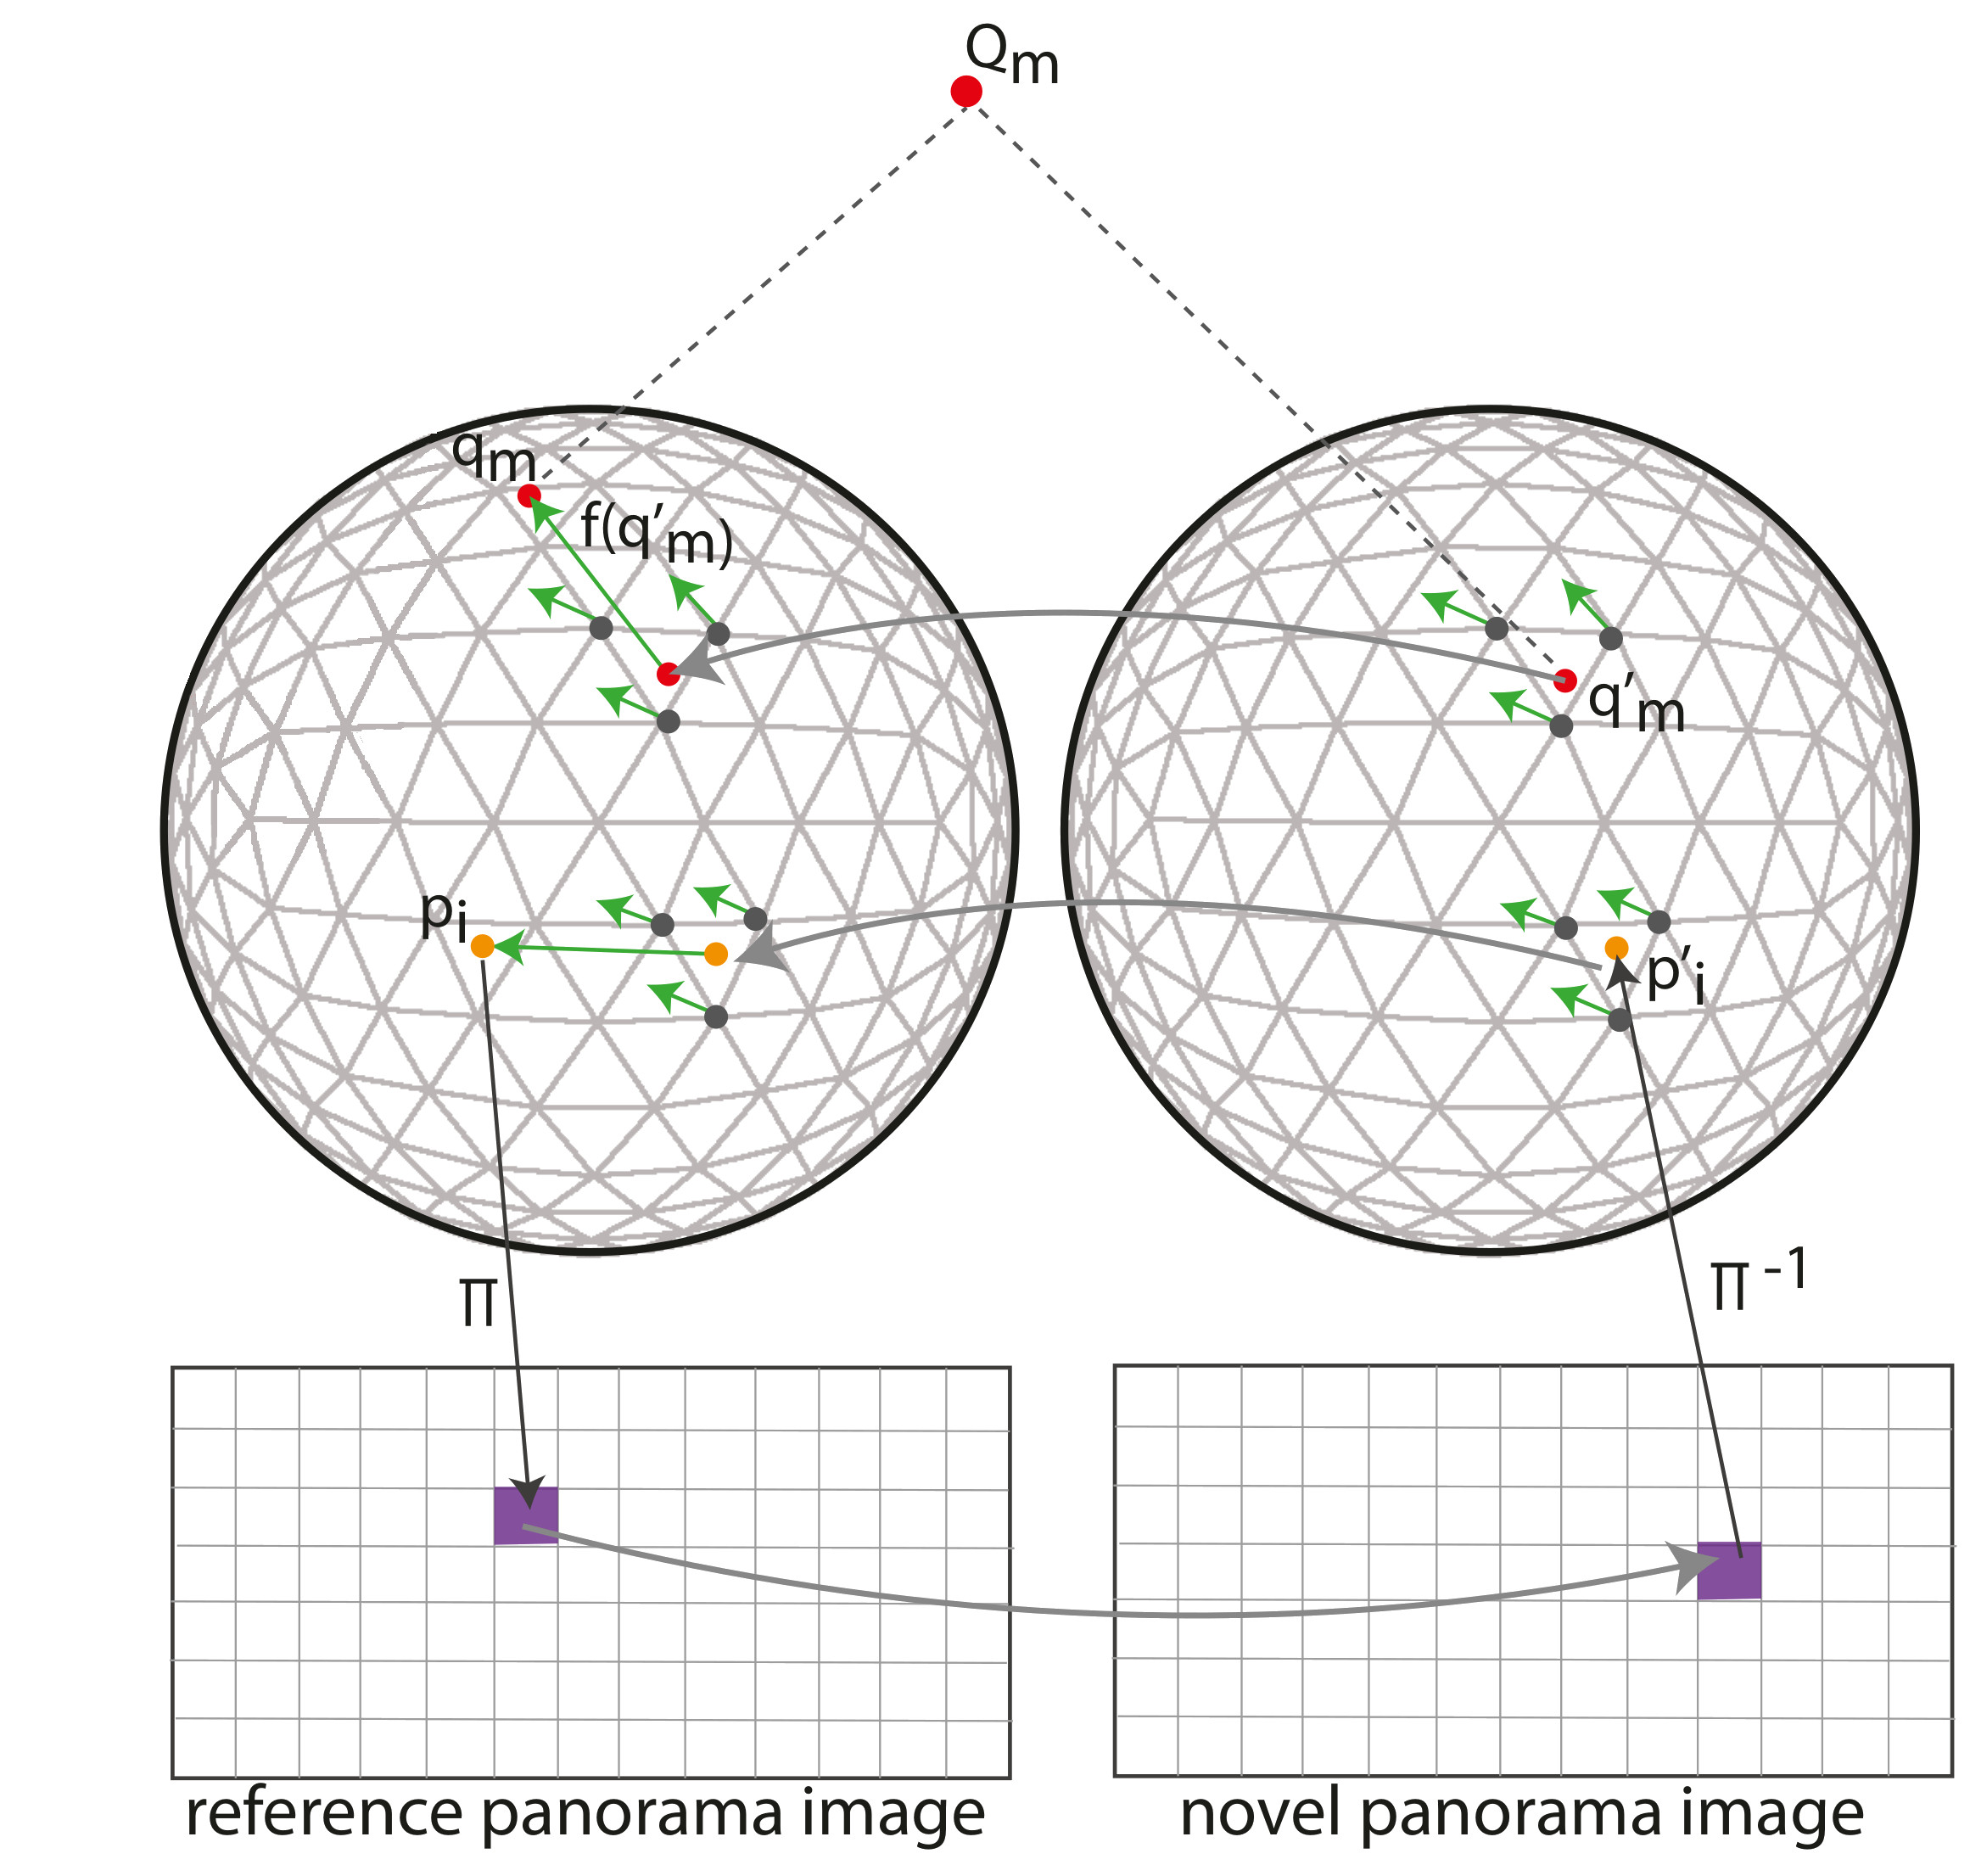
\includegraphics[width=0.6\textwidth]{02/6dof-figure.jpg}
\caption[Image warping from Huang et al.]{The warping field is computed by finding the movement between the projections of each 3D scene point in the reference and the synthesized frame. Then the warping field is used to map each pixel of the synthesized image to its corresponding pixel in the reference to look up its color information. \emph{Adapted from \cite{6dof}}}
\label{fig:6dof-figure}
\end{figure}

\subsubsection{Panorama Image Interpolation for Real-time Walkthrough}
correspondences needed: sparse, geometry: none, constraints: none, image rep: ?, type of warping: triangulation
Kawai et al.\ \cite{walkthrough} approach the problem of interpolating between images without using 3D geometry. Their basic setup is to capture four 360\degree images at each corner of a rectangular area and use their algorithm to interpolate within this area.

First, they manually select corresponding feature points in all four images, which they map to a sphere and triangulate. They create their synthesized mesh with bilinear interpolation, in which the triangulated meshes are deformed by using the Slerp (Spherical Linear Interpolation) function. To calculate the actual image, they use a combination of ray tracing and barycentric coordinates to get the uv coordinates of the synthesized image. Finally, the new image can be rendered by using the uv coordinates for texture mapping.

\subsubsection{On the Use of Ray-tracing for Viewpoint Interpolation in Panoramic Imagery}
correspondences needed: none, geometry: none/dense, constraints: color-constraint, image rep: cube, type of warping: pixel blending
Shi et al.\ \cite{raytracing} examine how ray tracing can be used to calculate arbitrary new viewpoints based on knowledge of relative positions between the viewpoints which are stored as cube maps. For every pixel in the target image, a ray is cast into the scene. At the point where the ray intersects with the scene, the rays from the reference images that also intersect with the scene at the same position, are calculated, yielding the corresponding point in the reference images.

Shi et al.\ introduce a color consistency constraint, which determines whether the pixel values of the reference images are similar. In areas where N reference images result in different colors, the pixel with the largest deviation is eliminated and the synthesized pixel is based on N - 1 reference pixels.

In order to calculate an intersection with the scene, they propose two different methods: A brute-force depth search which searches along the ray until the pixel values are similar enough to fulfill their color constraint requirements, or a guided depth search using sparse 3D reconstruction.

\subsubsection{Cube2Video: Navigate between Cubic Panoramas in Real-Time}
angular error metric
\end{comment}
